% Seccion de Diseno y construccion 

%%\chapter{Integración de componentes}
\section{Diseño y Construcci\'on}
\label{diseno}
El primer paso ha sido la construcci\'on de la parte física del robot. Para tal fin se procedió a la elección del diseño y ensamblaje de las piezas. En la sección \ref{subsection:diseno} se describe cada uno de los componentes utilizados para armar el robot, y luego, en la secci\'on \ref{subsection:construccion} se explica cómo se integraron esas piezas para obtener un humanoide adaptado a los objetivos de este proyecto.
\subsection{Diseño del robot}
\label{subsection:diseno}
%\label{subsection:componentes}
%\subsection*{Componentes de hardware}
A continuación se presenta una descripción de todos los elementos utilizados para la construcción del robot humanoide y sus decisiones de dise\~no. 

%\subsection*{Cuerpo del Robot}

Las opciones que se han consideradas para el cuerpo de Junny han sido: La construcci\'on con piezas de LEGO, la construcci\'on y dise\~no mec\'anico desde cero y la construcci\'on piezas del kit Bioloid. Estas opciones corresponden a los recursos disponibles. Tanto la construci\'on LEGO como la opci\'on de realizarlo desde cero implicaban mas tiempo del que se disponia, adem\'as que realizarlo en su totalidad con dise\~no mec\'anico y electr\'onico implicaba conocimientos m\'as avanzados en el \'area de mecatr\'onica que no eran el objetivo del proyecto. Por lo tanto la opci\'on m\'as factible para el cumplimiento de los objetivos es la construcci\'on con el kit Bioloid que es un kit de robótica con piezas prefabricadas que permite armar diferentes tipos de robot pero principalmente humanoides. Su empaque se puede observar en la figura ~\ref{fig:kit}. El fabricante, ROBOTIS, incluye un manual con varios modelos de robots con instrucciones de ensamblaje. Provee una tarjeta controladora, CM-510, a la que se conectan los motores Dynamixel y algunos sensores que se programan a través de la interfaz de ‘RoboPlus’\cite{robotics}. La tarjeta controladora CM-510 fue sustituida por la tarjeta controladora de software libre Arbotix. La utilización de la tarjeta Arbotix permite una mayor flexibilidad en el control de motores y la incorporación de una variedad de sensores no soportados por la tarjeta CM-510.
Además, la tarjeta Arbotix posee mayor soporte y amplitud en la comunicación entre distintos dispositivos, permite el control avanzado de algunos tipos de servos Dynamixel y robots basados en Bioloid. Incorpora un microcontrolador \gls{AVR}, radio inalámbrica \gls{XBEE}, conductores de motor dual, y cabeceras de estilo servo de 3 pines para entrada/salida digital y analógica \cite{arbotix}.

Los Motores Dynamixel Ax-12+ son actuadores inteligentes y modulares que incorporan un reductor de engranajes, un motor DC de presión y un circuito de control con funcionalidad de red lo cual permite formar series o cadenas de motores (figura ~\ref{fig:motoresDc}). Estos motores estan incorporados en el kit Bioloid al igual que la batería de polímero de litio (Lipo) una fuente de poder usada para motores y componentes electr\'onicos. La batería usada es de 11.1 voltios y 1 amperio. \cite{bateria}




%\begin{figure}[hbtp]
%\centering
%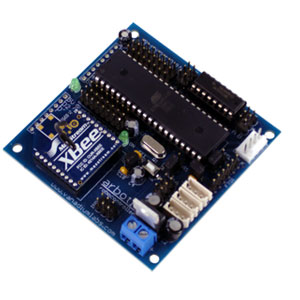
\includegraphics[scale=0.5]{imagenes/ARBOTIX.JPG}
%\caption{Tarjeta controladora ArbotiX}
%\end{figure}

\begin{figure}[hbtp]
\centering
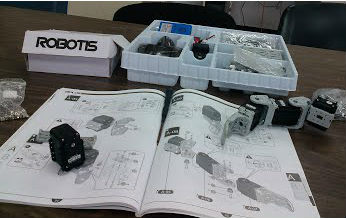
\includegraphics[scale=0.5]{imagenes/kitAfuera.jpg}
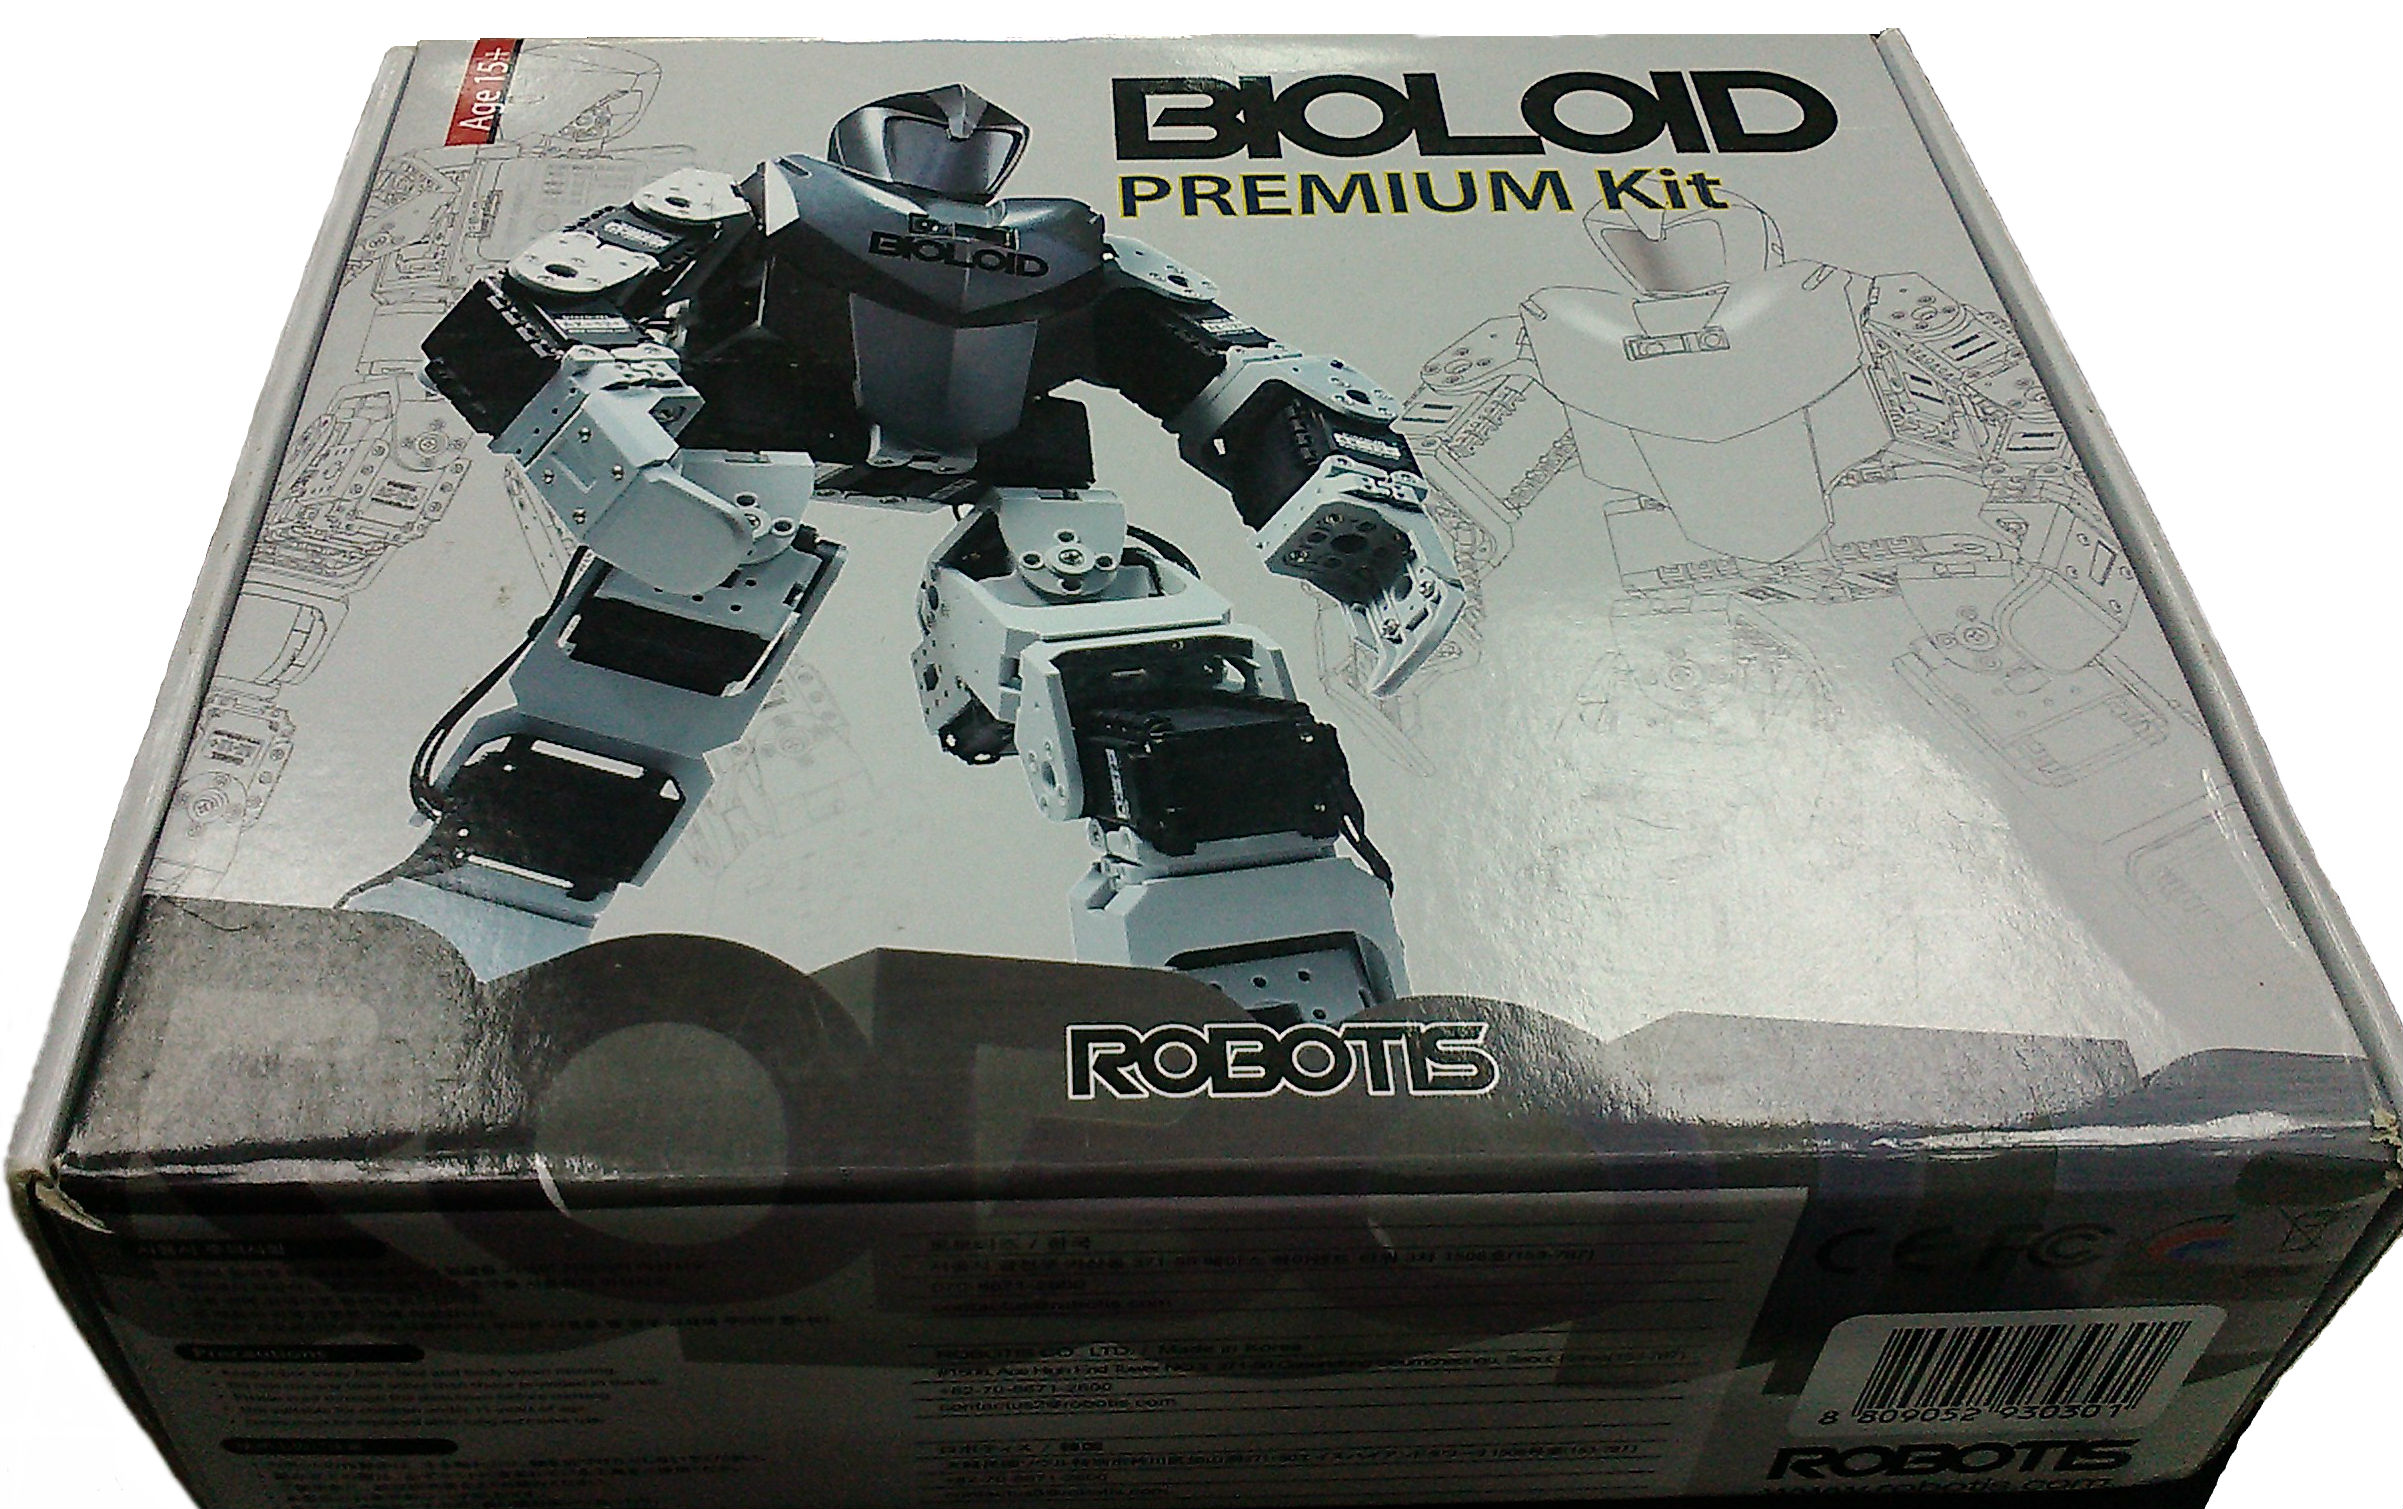
\includegraphics[scale=0.07]{imagenes/cajaKit.jpg}
\caption{Bioloid Premium Kit}
\label{fig:kit}
\centering
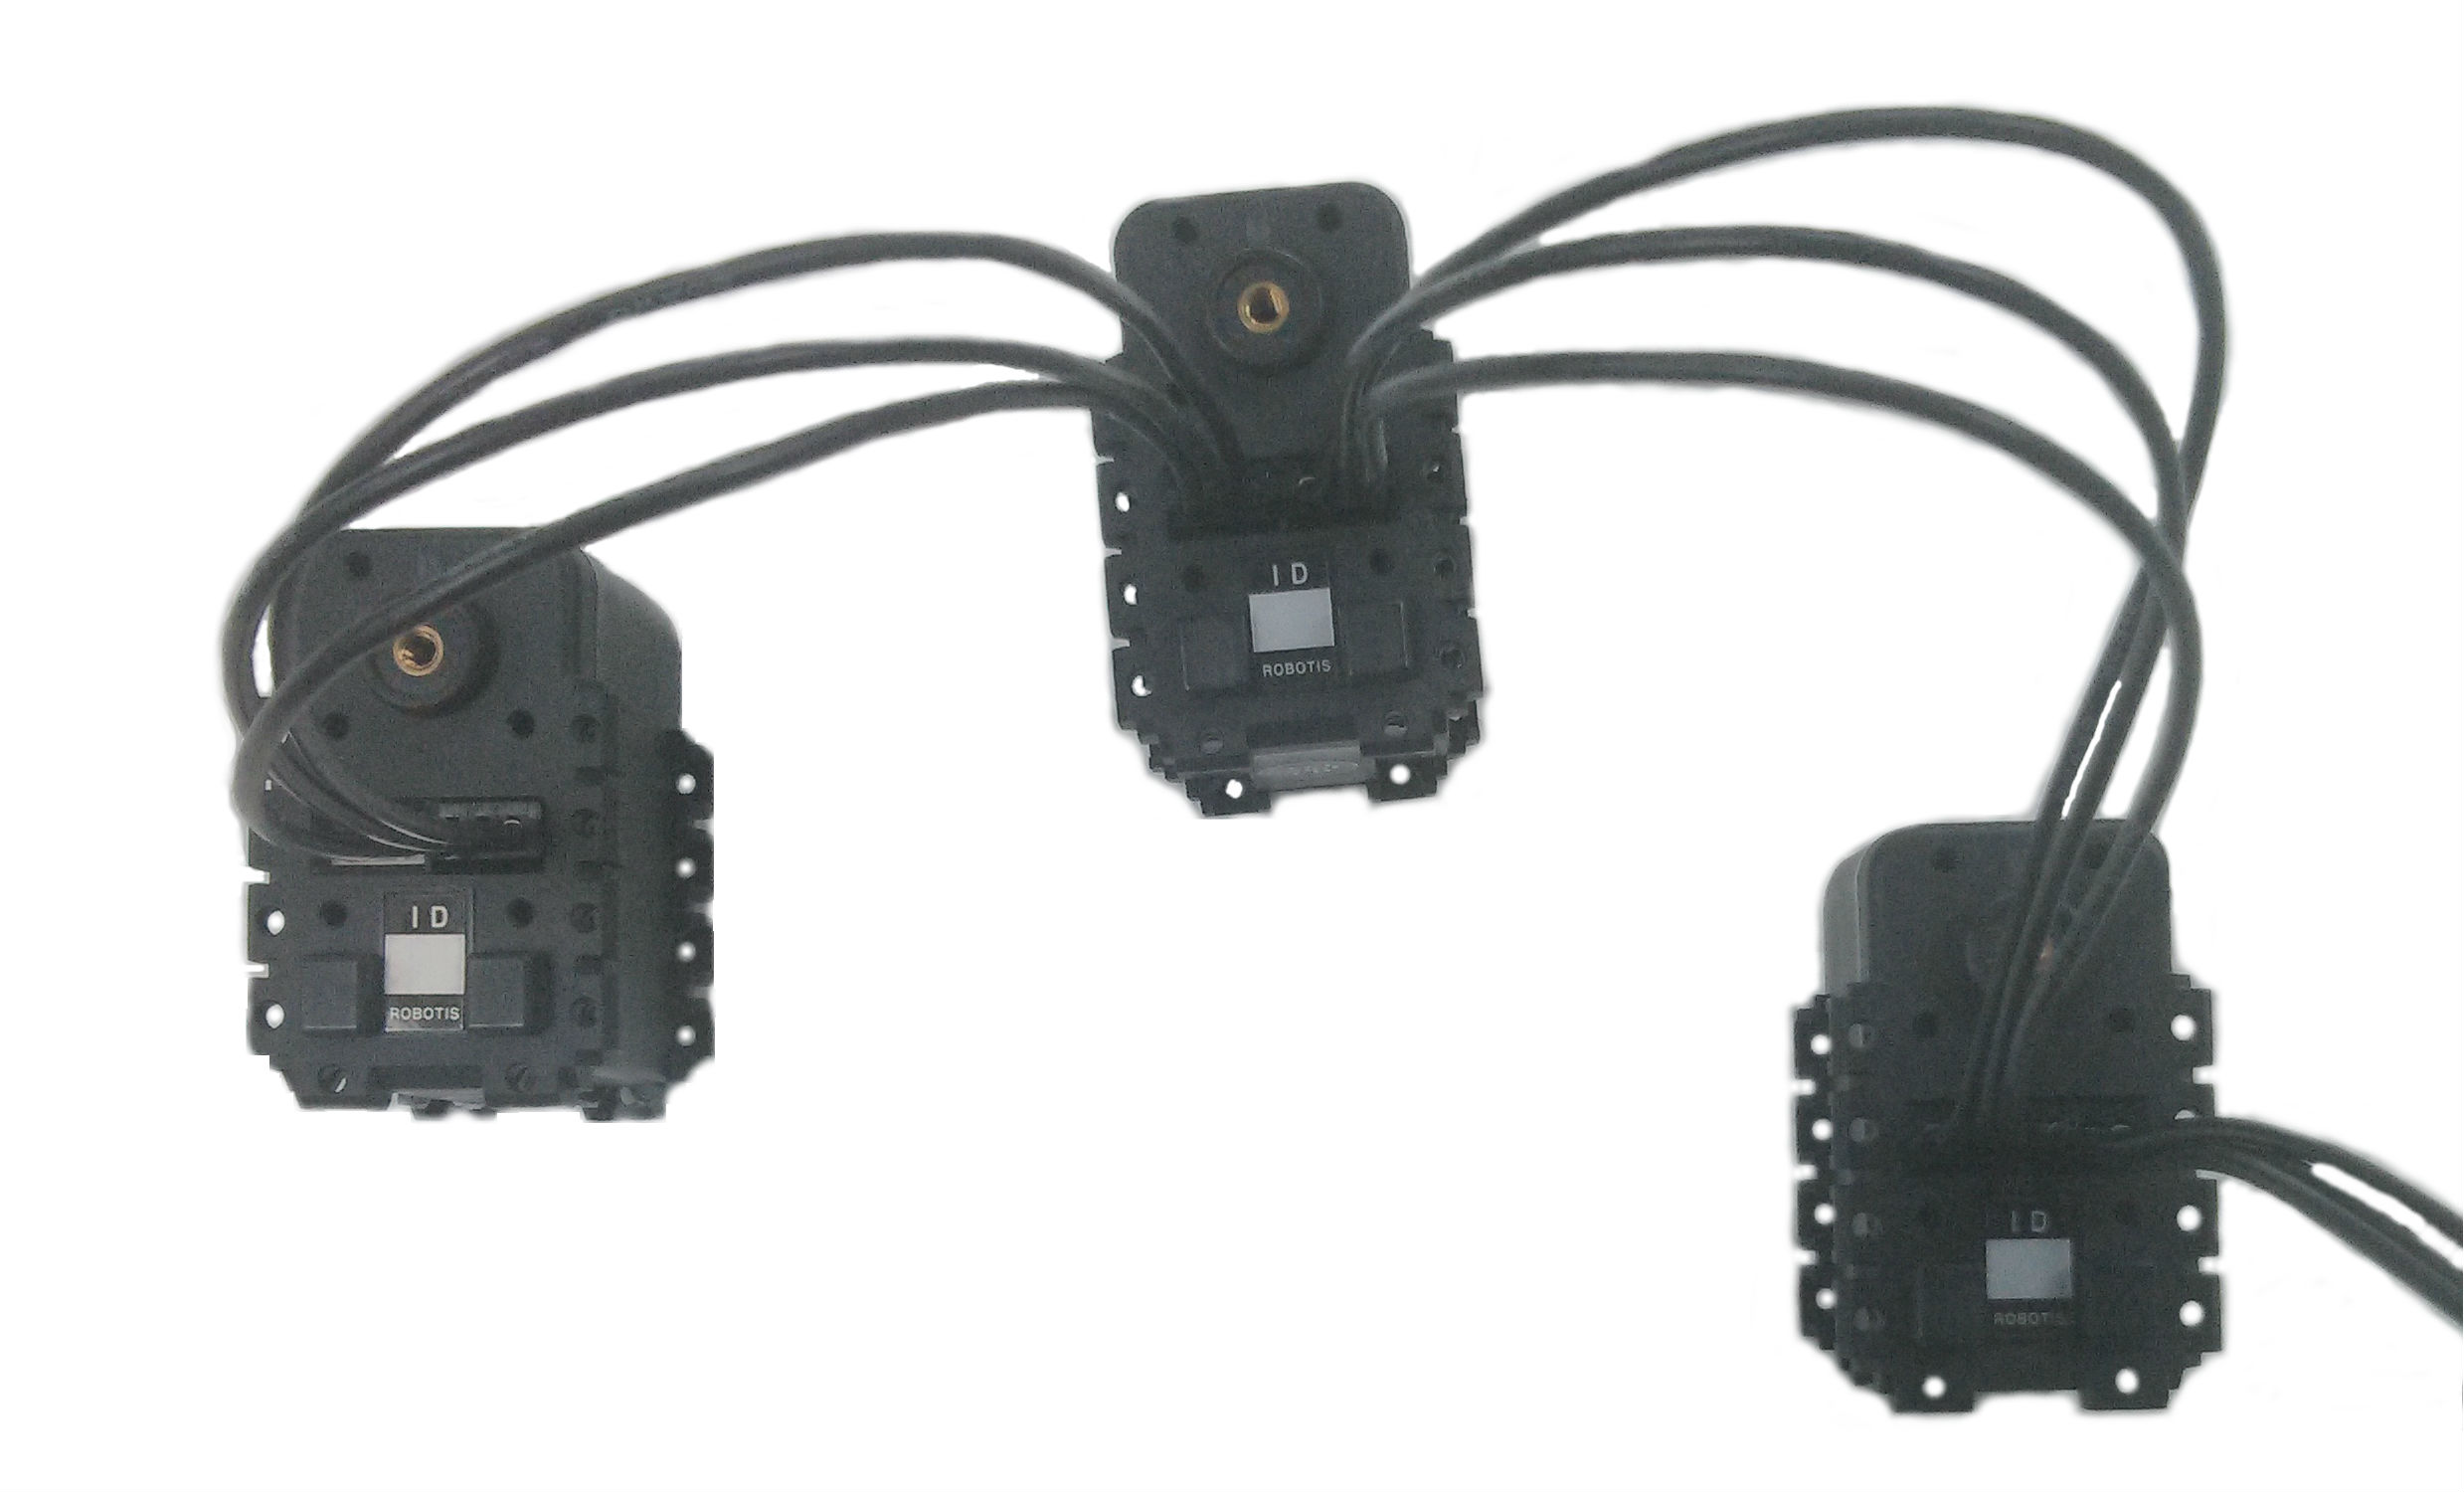
\includegraphics[scale=0.1]{imagenes/3Dynamixel.jpg}
\caption{Motores Dynamixel conectados en serie}
\label{fig:motoresDc}
\centering
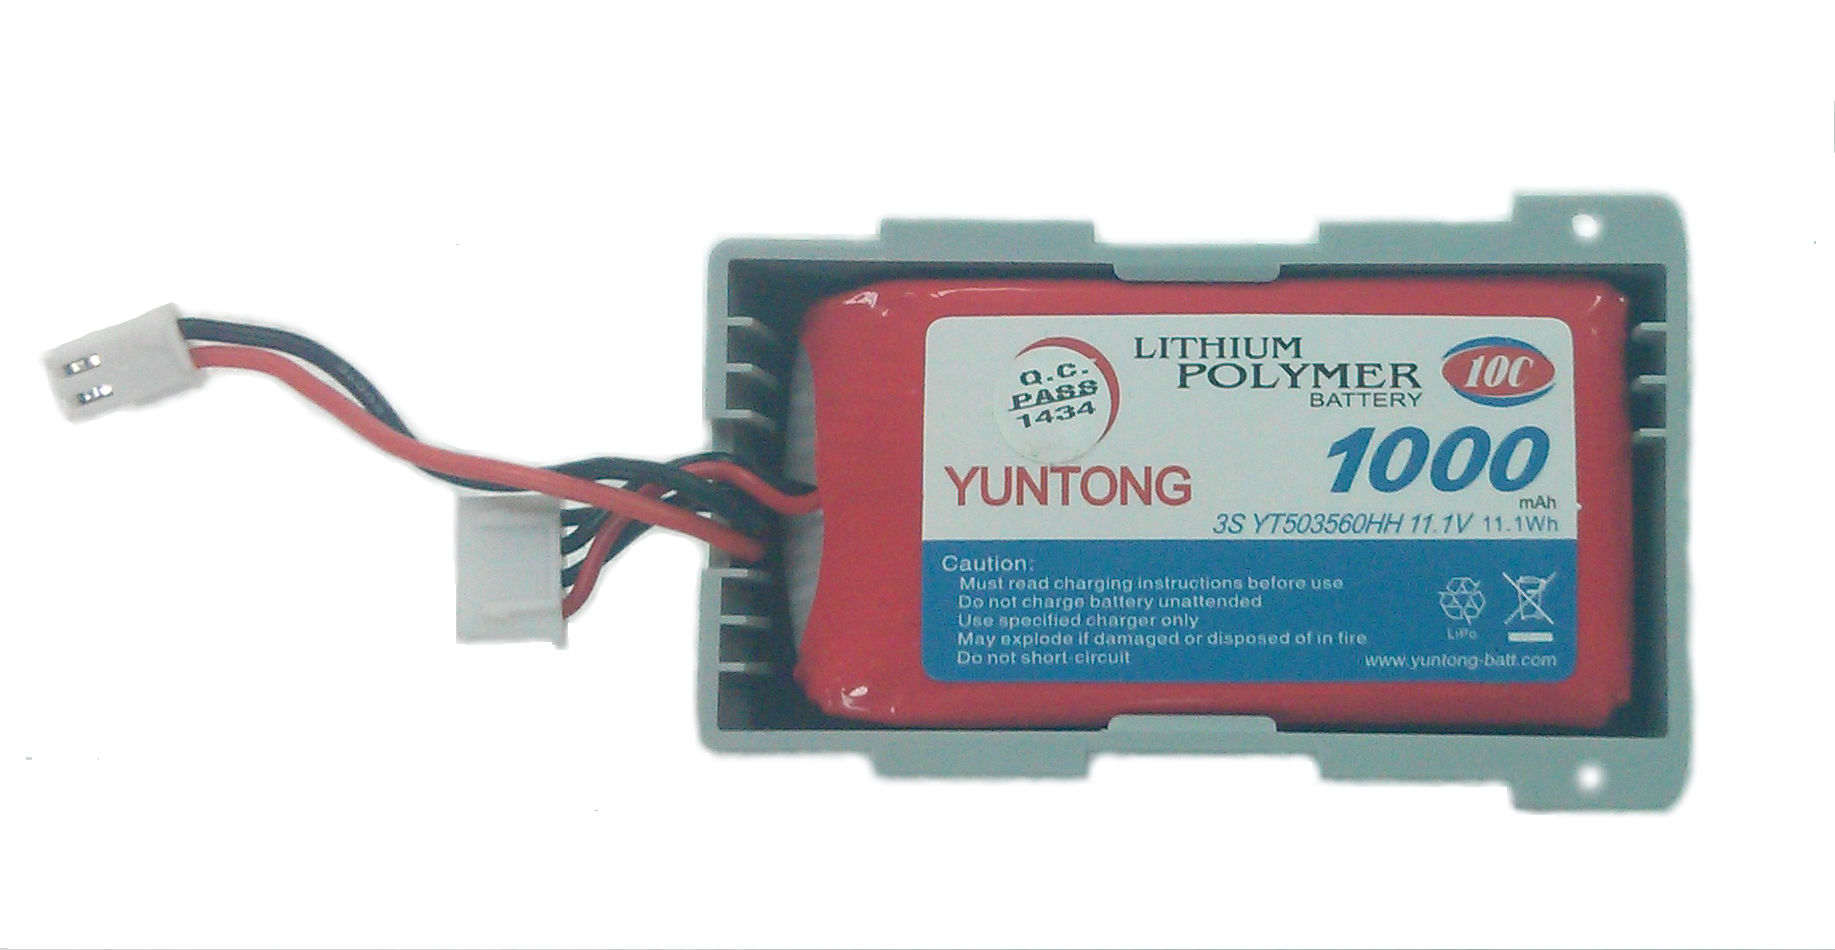
\includegraphics[scale=0.1]{imagenes/bateriaLipo.jpg}
\caption{Batería Lipo}
\label{bateria}
\end{figure}

%\begin{figure}[hbtp]


%\end{figure}

Para el balance y detecci\'on de ca\'idas de Junny se utiliz\'o con un giroscopio (Robotics Gyro) que mide la velocidad angular que genera los movimientos del robot, este se encuentra diseñado para mantener el balance del robot y ser usado para otras aplicaciones de movimiento\cite{gyro}. En figura ~\ref{fig:gyro} se puede observar su estructura. Existen otros sensores de inercia que se enfocan en realizar la tarea de balance y orientaci\'on del robot como el aceler\'ometro.



El FTDI (Future Technology Devices International) utilizado para comunicar fisicamente a la Arbotix y a la Raspberry Pi  es una tarjeta controladora  (figura ~\ref{fig:ftdi}) que ofrece el servicio de conversión de  datos de USB a UART. Permite la comunicación entre diferentes dispositivos \cite{ftdi} fue elegida en lugar de XBEE pues la Raspeberry Pi y Arbotix estan fisicamente cerca y usar XBEE implicaba un mayor costo para el proyecto.


\begin{figure}[hbtp]
\centering
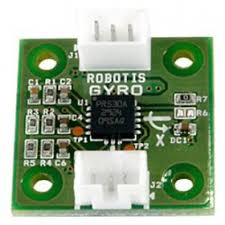
\includegraphics[scale=0.35]{imagenes/gyro.jpg}
\caption{Sensor Gyro}
\label{fig:gyro}
\centering
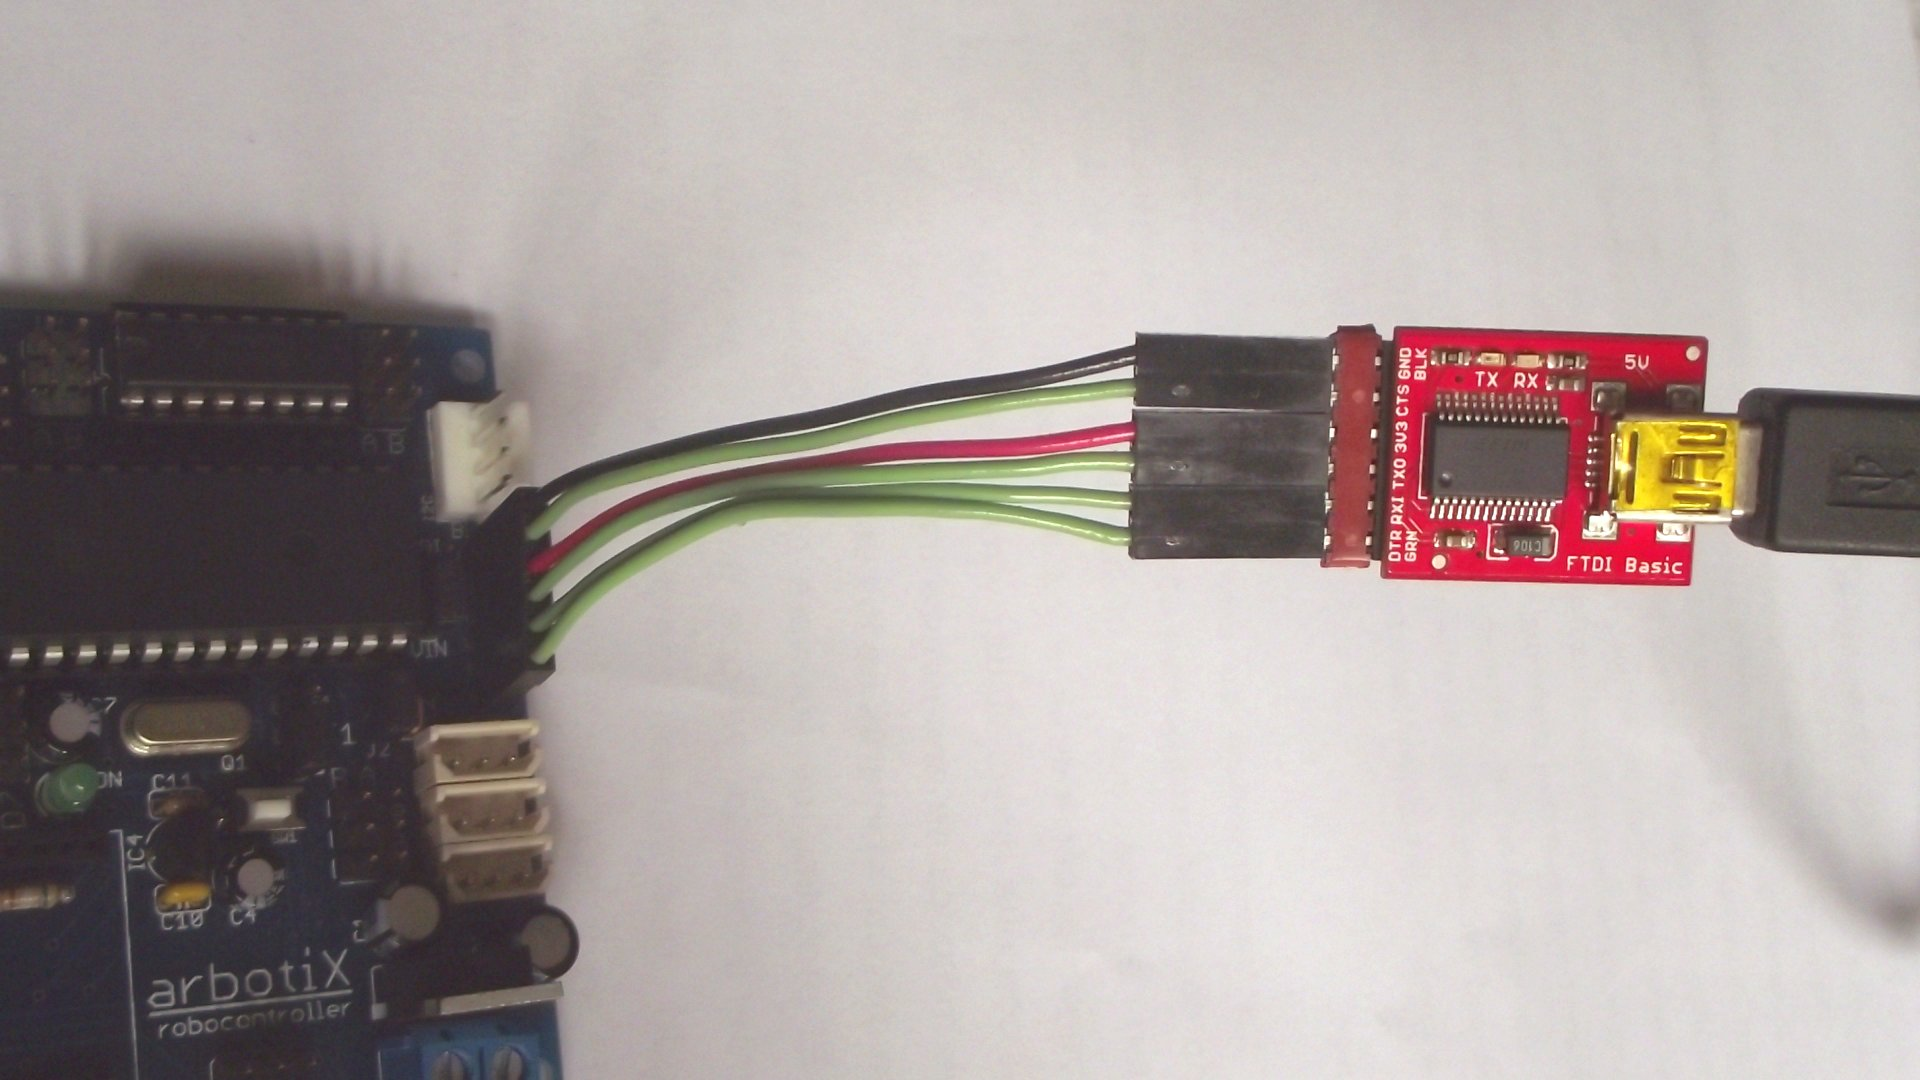
\includegraphics[scale=0.06]{imagenes/DSCF1162.jpg}
\caption{Chip FTDI conectado a la tarjeta Arbotix}
\label{fig:ftdi}
\centering
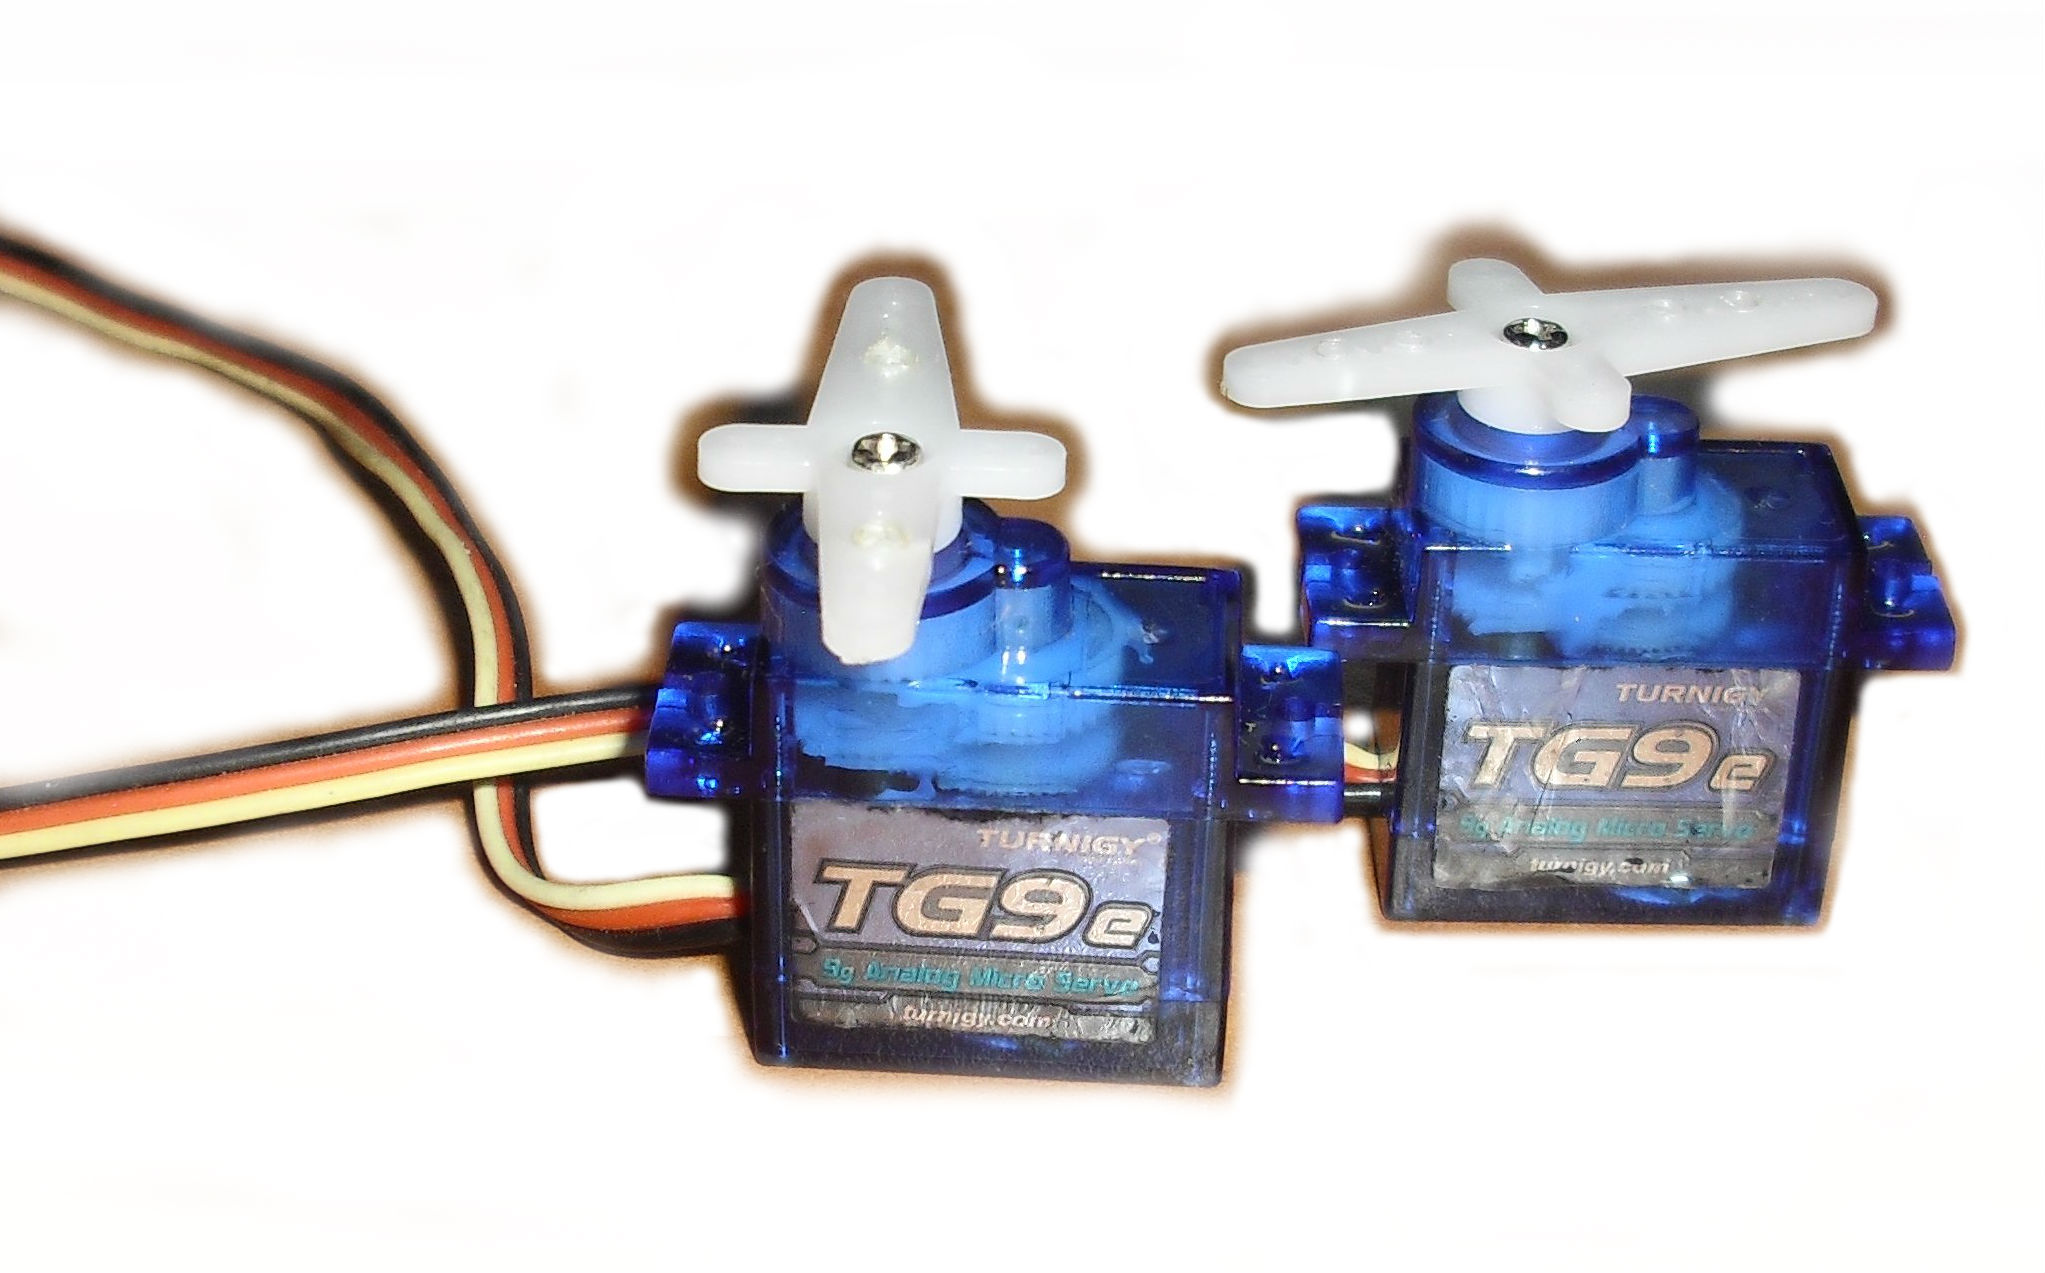
\includegraphics[scale=0.09]{imagenes/servosTg9B.jpg}

\caption{Micro Servomotores analógicos TG9e}

\label{fig:Servo}
\end{figure}


El extensor de puertos Bioloid fue necesario para una mejor movilidad del robot se dividi\'o su cuerpo en cuatro extreminades por lo tanto cuatro series de motores distintas y el expansor permite aumentar el número de cadenas de servos conectados a la tarjeta (ver figura ~\ref{fig:ext}) \cite{hub}.
De igual manera es explicado a m\'as profundidad en la siguiente secci\'on.


\begin{figure}[hbtp]
\centering
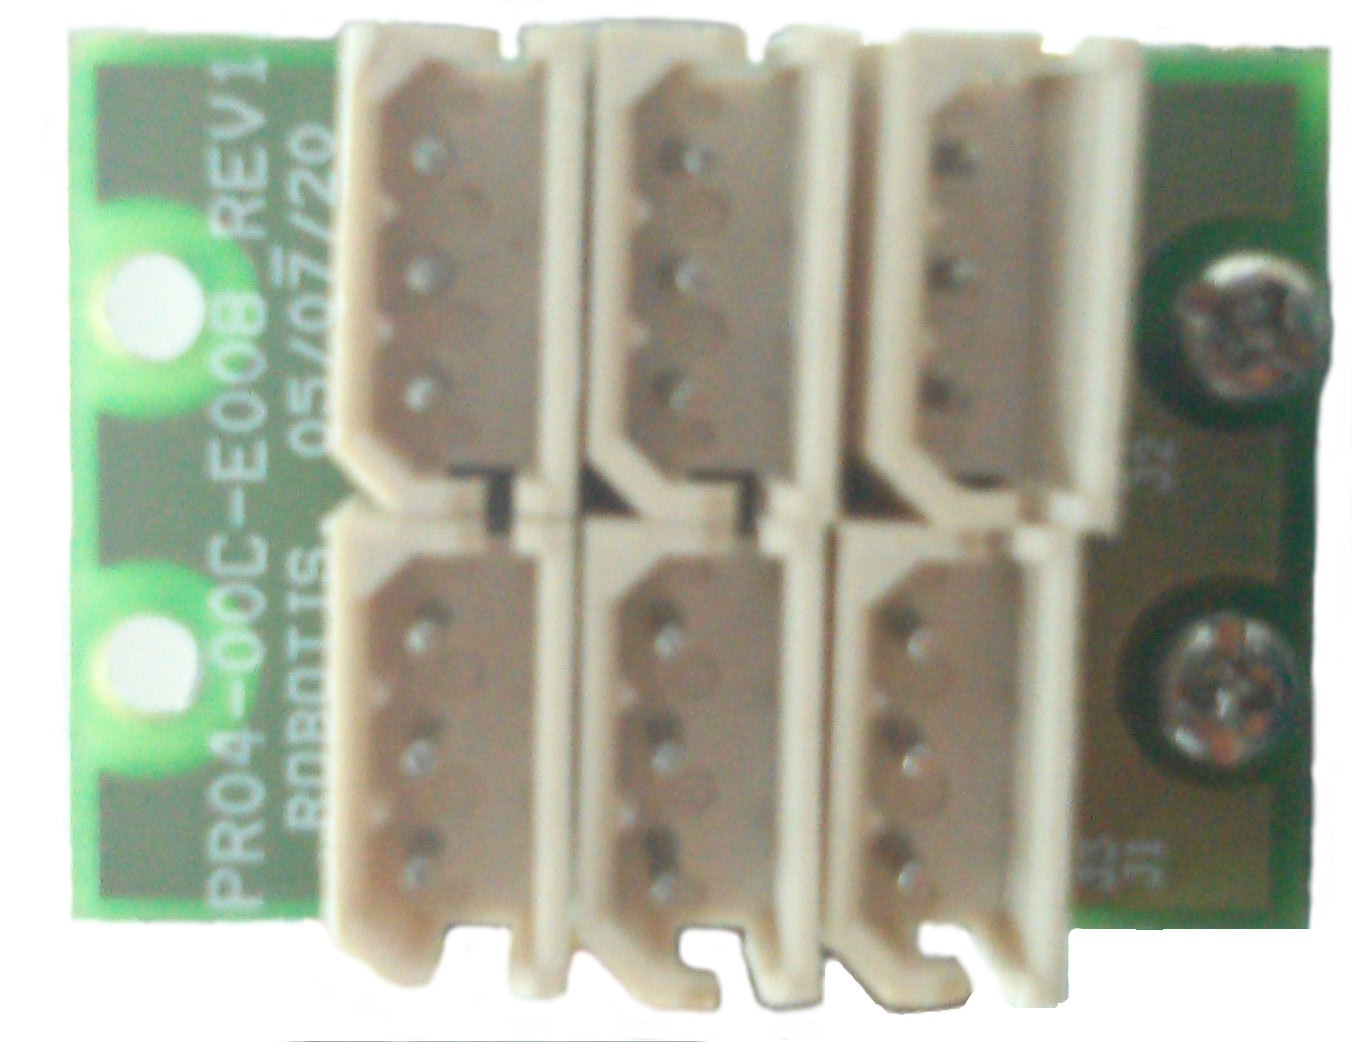
\includegraphics[scale=0.08]{imagenes/extensor.jpg}
\caption{Extensor de puertos Bioloid}
\label{fig:ext}
\end{figure}
 
Para el movimiento de la c\'amara se utiliza como base dos micro servo motor anal\'ogico TG9e que es un pequeño servomotor cuya capacidad de torque alcanza los 1.50 kg-cm \cite{microservo}. Permite ser controlado en posición en un rango de 180$^{\circ}$. Ver figura ~\ref{fig:Servo}.   

La Raspberry Pi es un computador de aproximadamente 10 cm de largo, a la que se puede conectar un monitor y un teclado. Puede ser utilizado en proyectos de electrónica y para varias de las tareas que un computador de escritorio puede hacer, como hojas de cálculo, procesadores de texto y juegos \cite{raspberry}. Ver figura ~\ref{fig:Raspe}. La Raspberry Pi cuenta con un procesador gráfico que permite aligerar la carga del procesador central \cite{elLinux}. Para las funciones correspondientes a la Rasberry Pi, en el proyecto tambi\'en era factible la utilizaci\'on de un tel\'efono celular avanzado, sin embargo esta opci\'on fue decartada pues la c\'amara del tel\'efono no posee grados de libertad, agrega un peso importante a la estructura del robot y un costo superior que la utilizaci\'on de la raspberry.  



%imagen tomada de: %http://rayhightower.com/blog/2012/12/03/ruby-on-raspberry-pi/
\begin{figure}[hbtp]
\centering
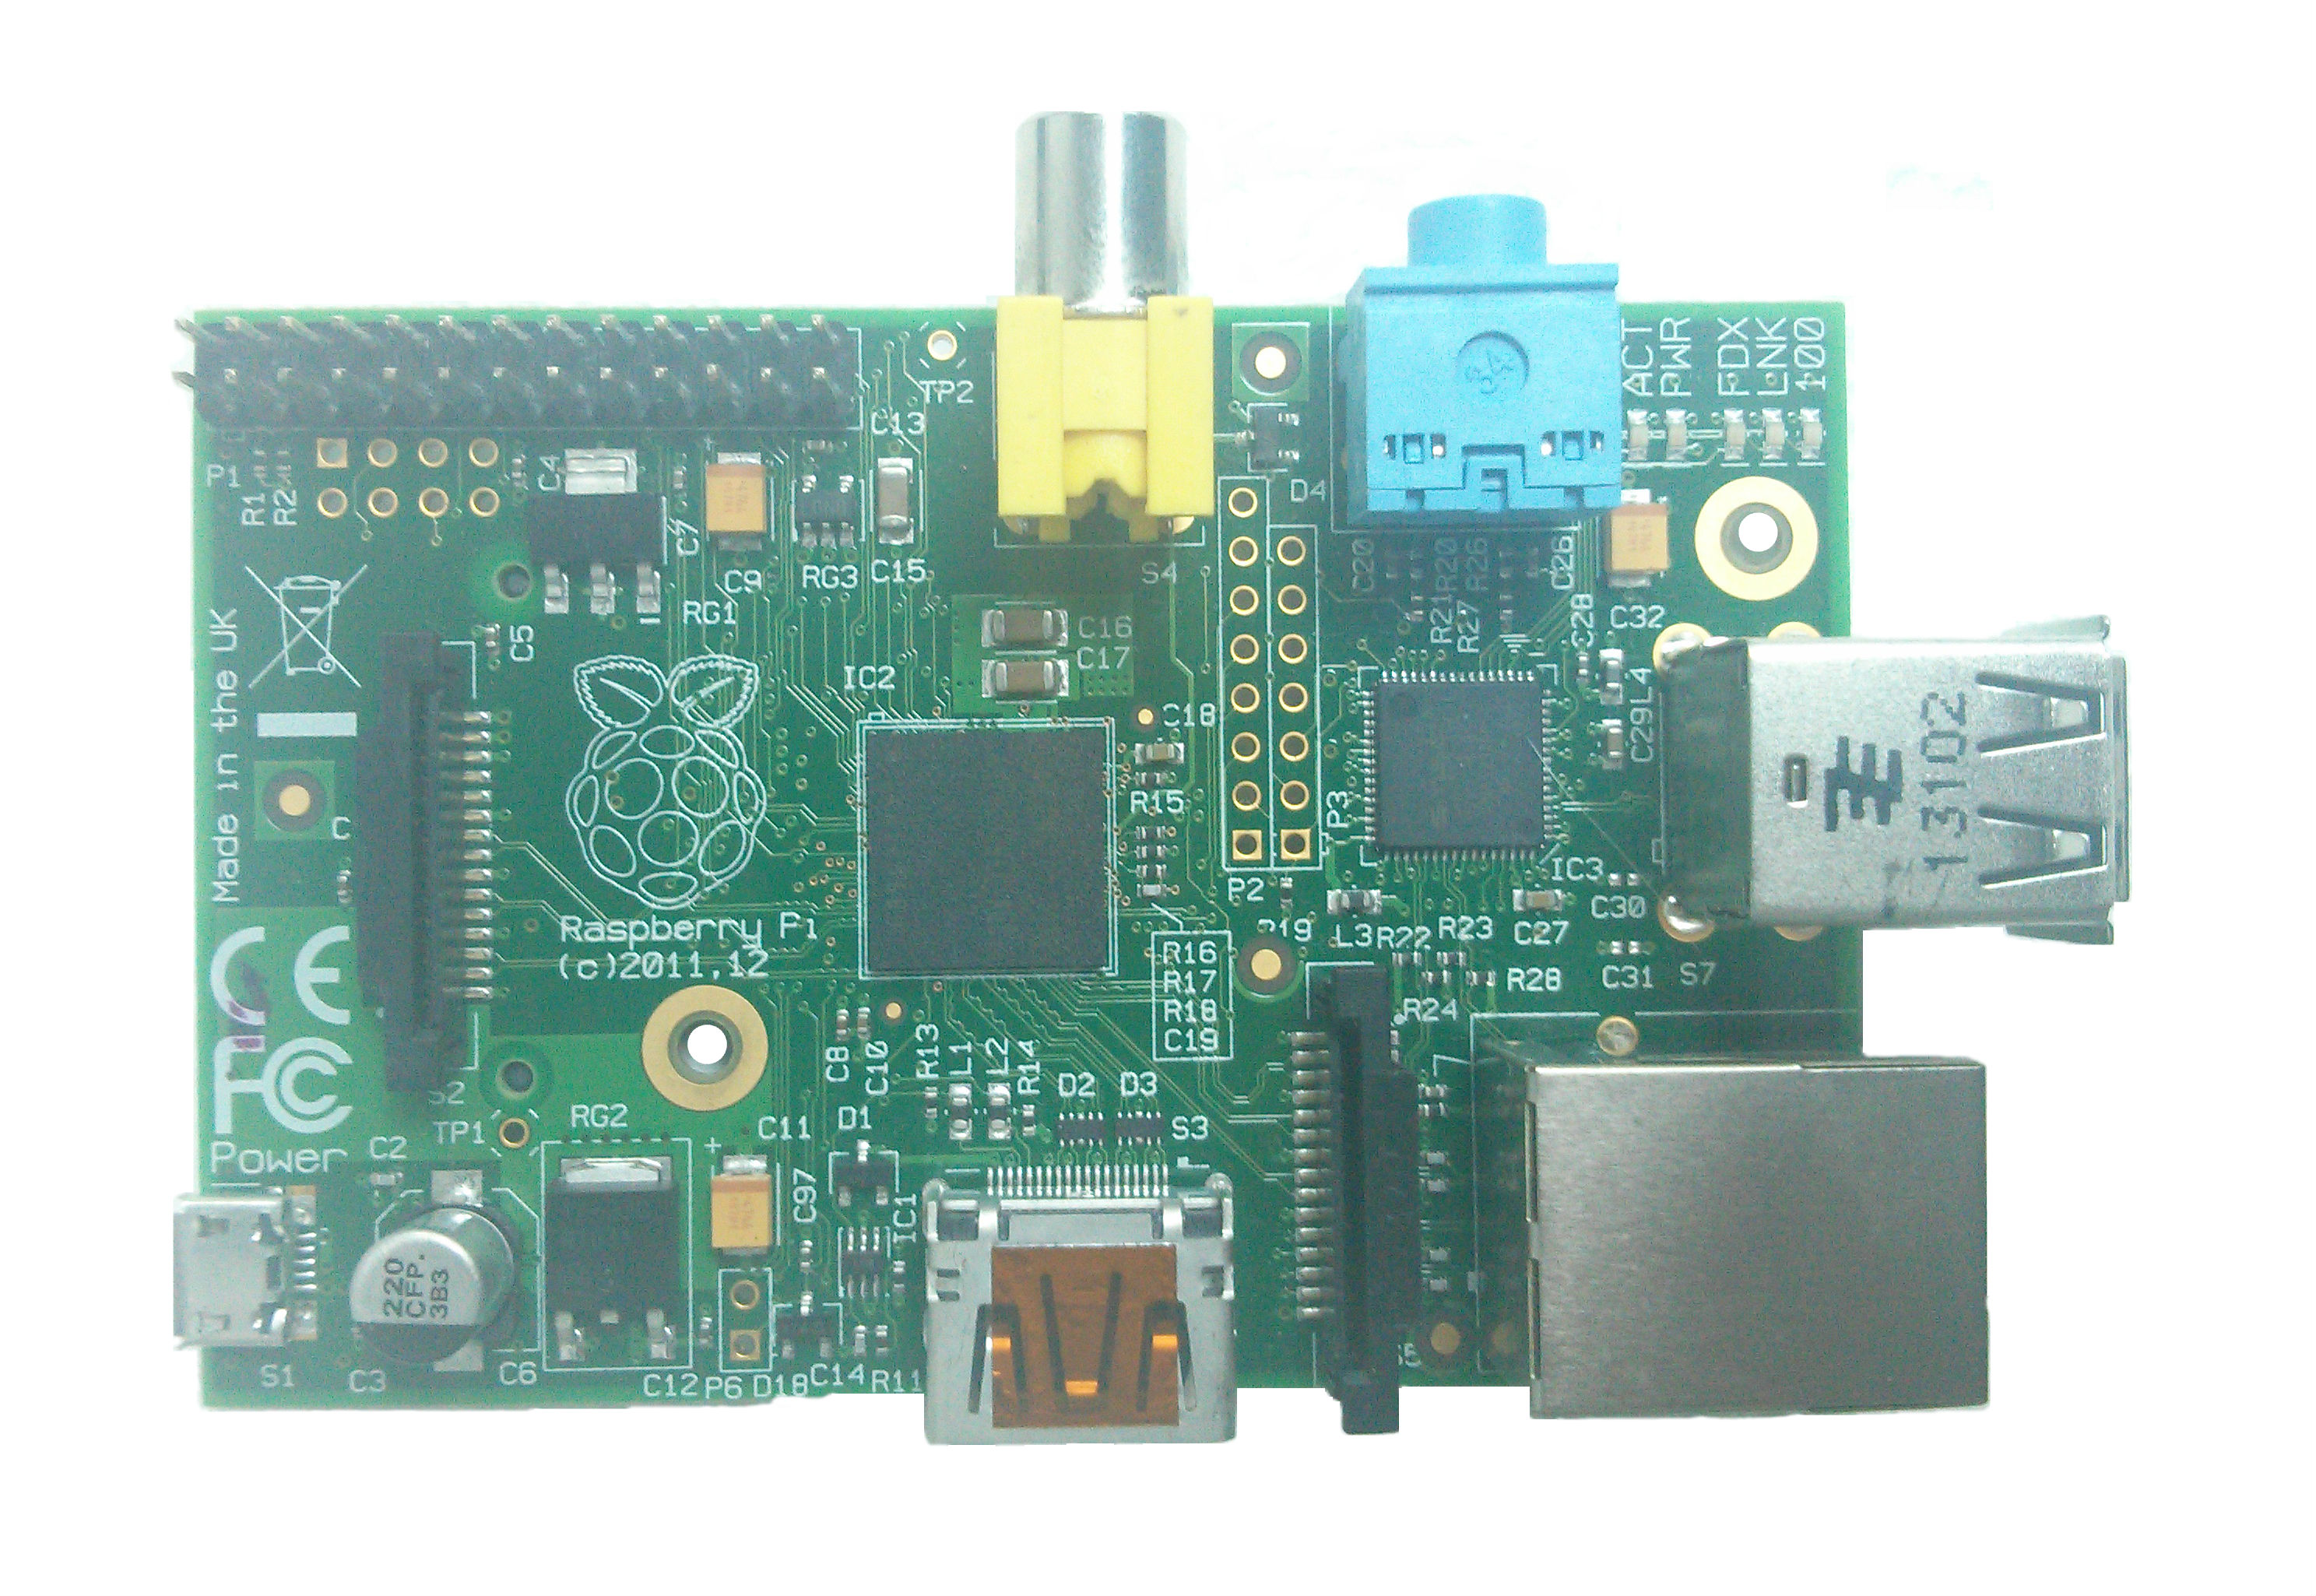
\includegraphics[scale=0.06]{imagenes/RaspberryPi.jpg}
\caption{Tarjeta Raspberry Pi}
\label{fig:Raspe}
\centering
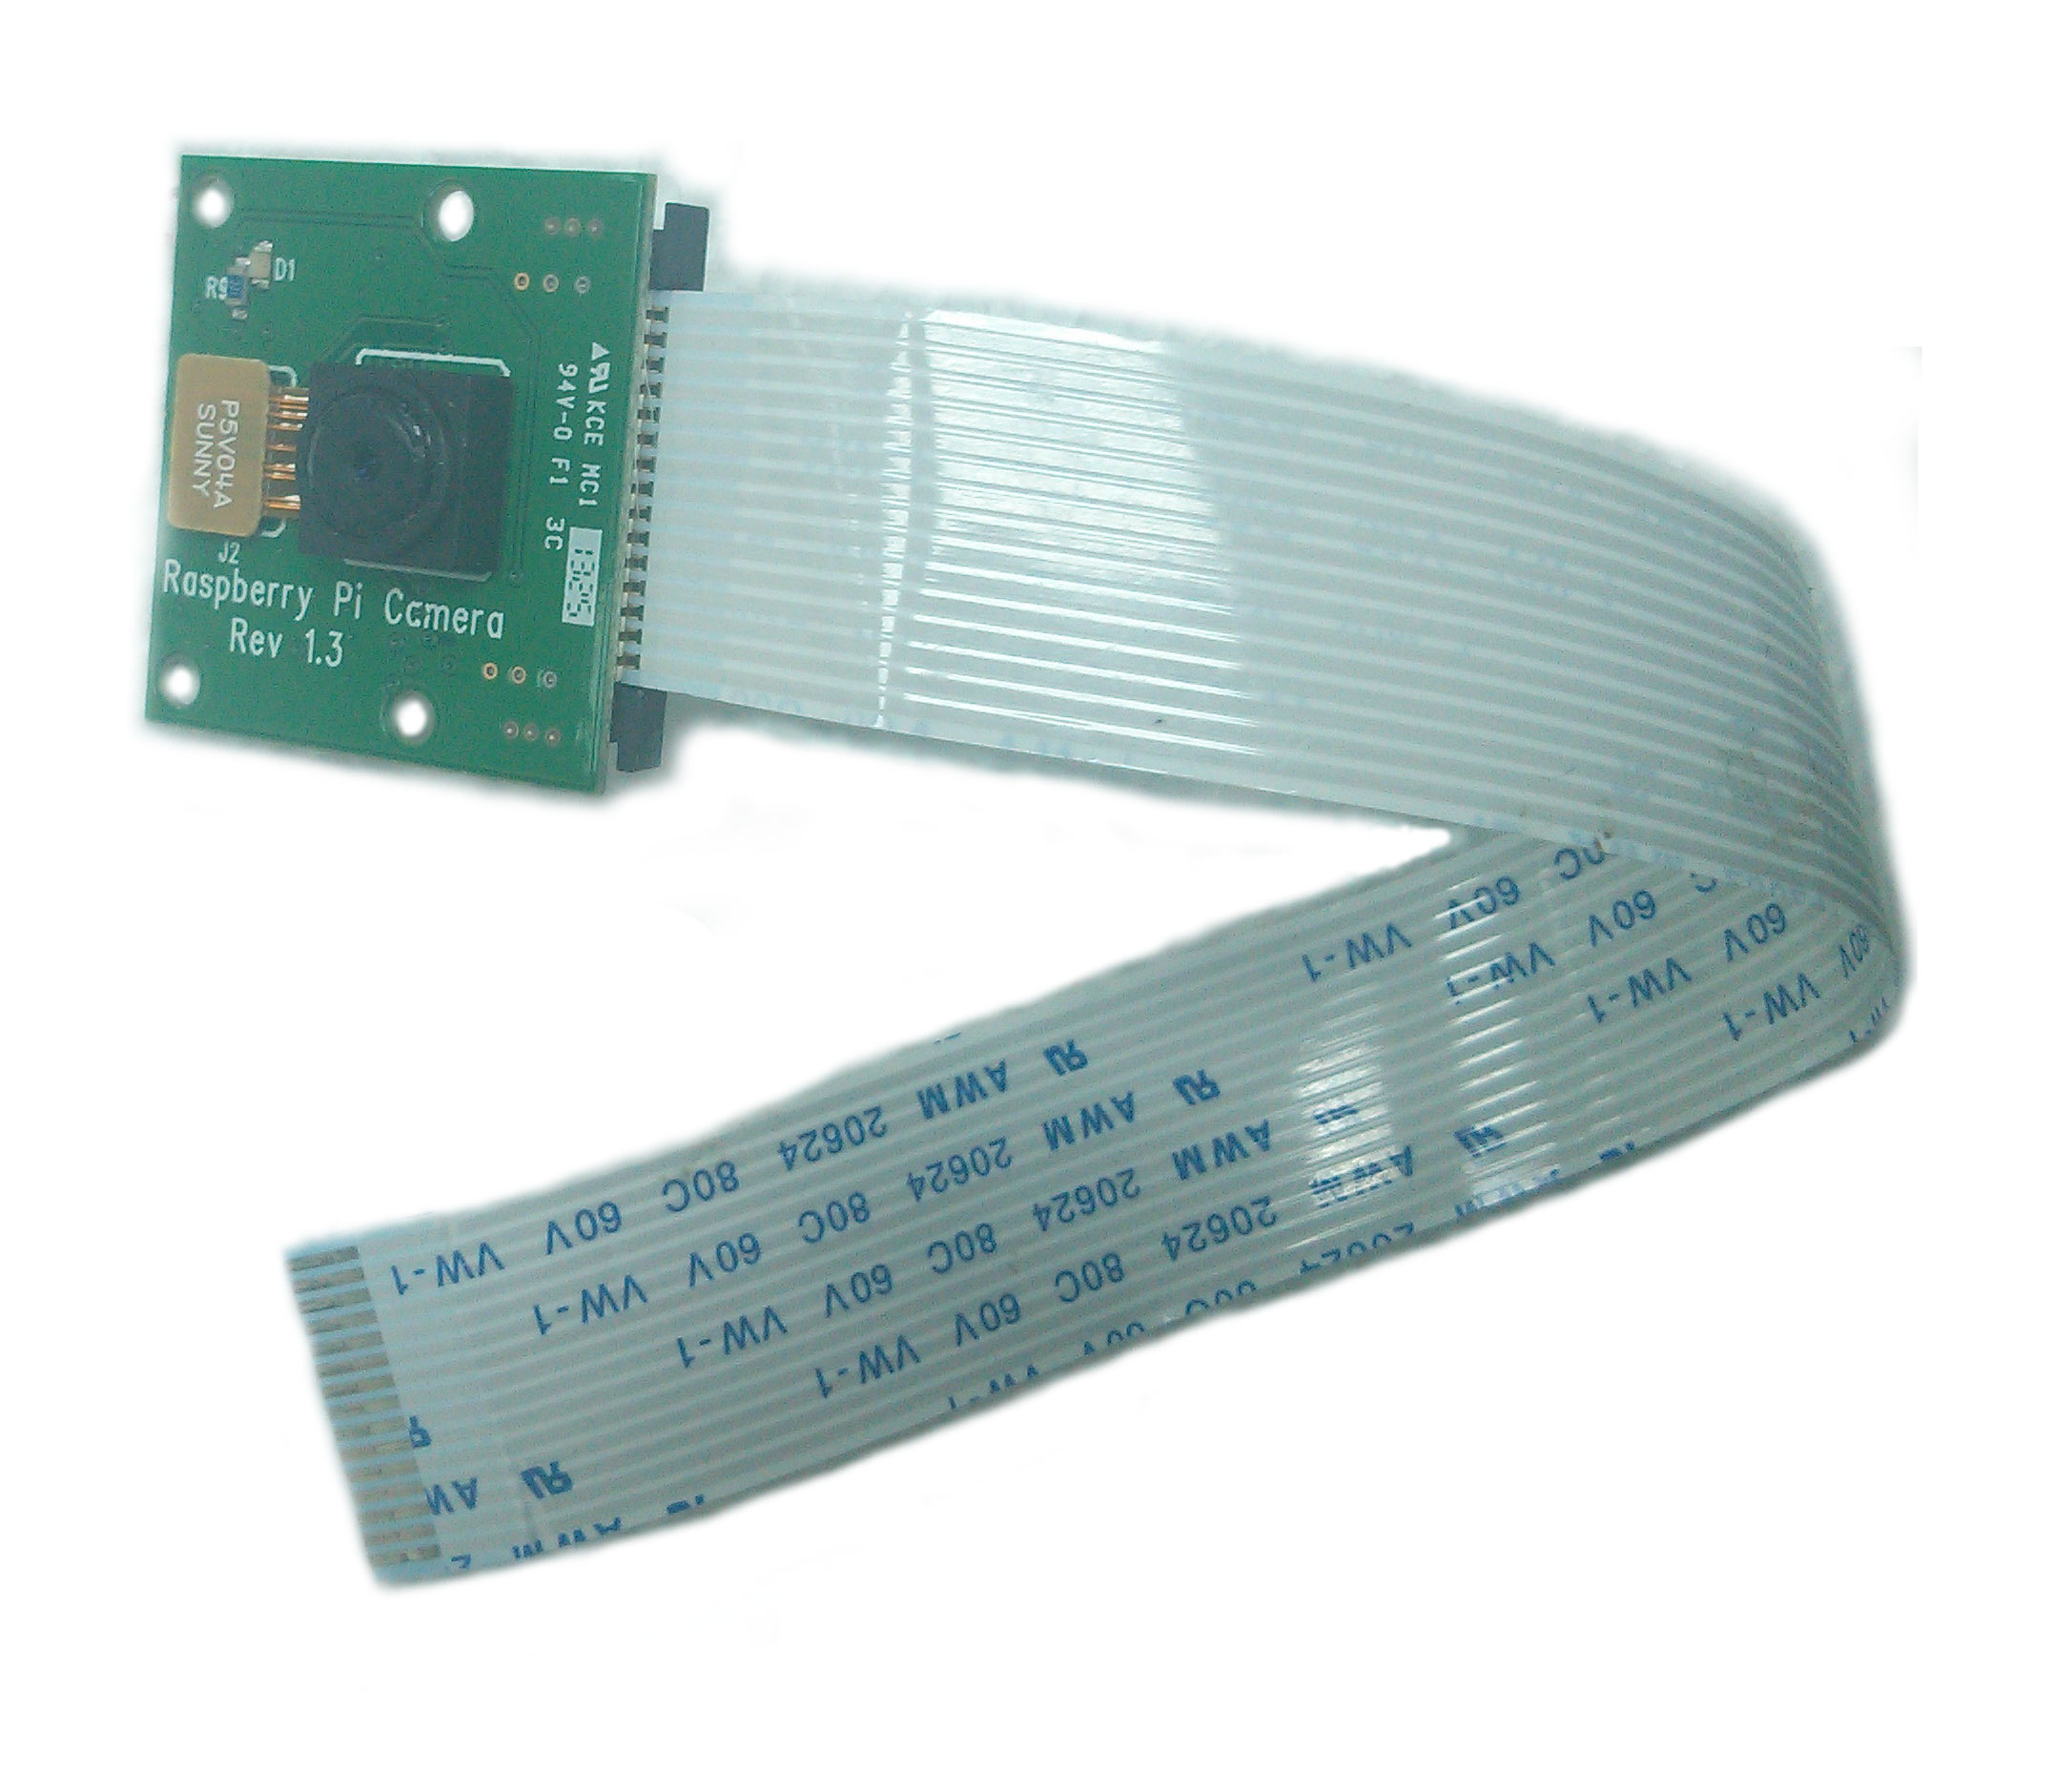
\includegraphics[scale=0.06]{imagenes/CamRasp.jpg}
\caption{C\'amara Raspberry Pi}
\label{fig:came}
\end{figure}

Para lograr el objetivo de detecci\'on de la pelota y orientaci\'on al arco existen varias posibilidades factibles para la tarea, un sensor de br\'ujula, un sensor de proximidad, entre otros, sin embargo la ulitizaci\'on de una c\'amara para esta tarea representaba numerosas ventajas como la certeza de ubicar la pelota, presi\'on en la distancia, el ahorro de la utilizaci\'on y manejo de mas sensores y la posibilidad de ampliar las habilidades y tareas que podr\'ia realizar Junny. Por ello se tomo la elecci\'on de la     
c\'amara Raspberry Pi que puede captar im\'agenes y grabar vídeos de alta definición. Se conecta a la Raspberry Pi con un cable de cinta plana de 15 cm en el puerto CSI. Tiene 5 megapíxeles de foco fijo que soporta los modos de vídeo de 1080x30, 720x60 y VGA90. Puede ser manejada con las librerías MMAL, V4L u otras librerías de terceros como la de Python \cite{raspberrycam}.(figura ~\ref{fig:came})  %(http://www.raspberrypi.org/products/camera-module/)

Debido a que no todos los componentes poseen las mismas exigencias con respecto a voltaje y amperaje, se realizó un regulador (ver figura ~\ref{fig:circuito}) con una salida de 5 voltios para la tarjeta Raspberry Pi y dos micro servomotores, y otra salida de 11.1 V para la tarjeta Arbotix que a su vez alimenta a los componentes conectados en ella (motores Dynamixel y Giroscopio). Si bien la tarjeta Arbotix posee un regulador interno de cinco voltios la opción de conectar todo a la salida de 5 V del regulador no era posible, dado que los motores Dynamixl requieren alimentación de 11 voltios.

\begin{figure}[hbtp]
\centering
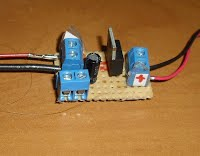
\includegraphics[scale=0.5]{imagenes/circuito.jpg}
\caption{Circuito con entrada de 11.1 V. Una salida de 5 V para los micro servomotores anal\'ogicos y tarjeta Raspberry Pi. Otra salida de 11.1 V para alimentar la controladora Arbotix.}
\label{fig:circuito}
\end{figure}

%\begin{figure}[hbtp]
%\centering
%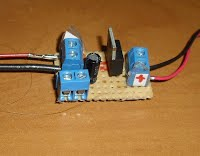
\includegraphics[scale=0.7]{imagenes/circuito.jpg}
%\caption{Lipo}
%\end{figure}

\label{subsection:construccion}
\subsection{Construcción}
Como se menciono anteriormente para la construcción del robot se utilizó el kit de piezas Bioloid Premium de marca Robotis el cual incluye motores Dynamixel Ax-12+, una tarjeta controladora CM-510, un sensor Gyro, un manual, entre otros elementos. El manual incluye las instrucciones de como armar los modelos A, B y C de humanoide, el utilizado en este proyecto es el tipo B, haciendo uso de 16 motores. En las figuras ~\ref{fig:frontal} y ~\ref{fig:trasera1} se puede observar la estructura del robot que aparece en el manual del kit. La elecc\'ion de este modelo se debi\'o a que los motores como recuersos eran escasos y este modelo al igual que el modelo C utiliza dos motores menos que el modelo A, ya que el A combina los grados de liberdad en la cadena que los modelos B y C poseen por separado. El modelo B posee un grado de libertad de interes a la hora de girar del robot por ello se eligi\'o en particular.

\begin{figure}[hbtp]
\centering
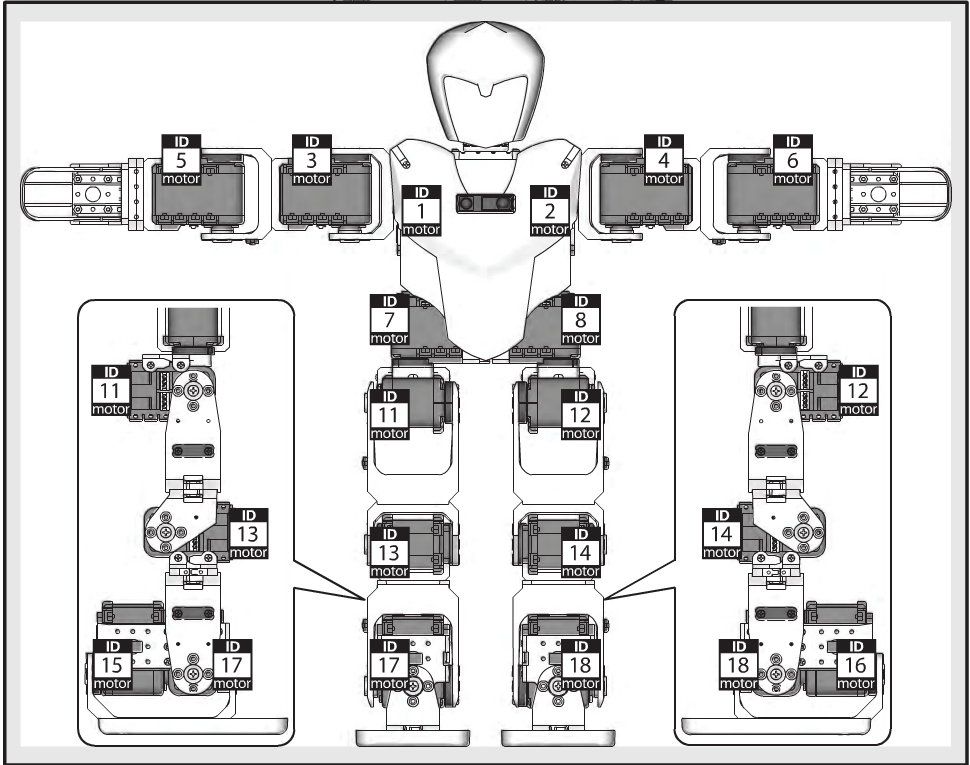
\includegraphics[scale=0.3]{imagenes/Robot.png}
\caption{Vista frontal del robot, tipo B, tomada del manual. Se puede apreciar la identificación ‘ID’ de cada motor Dynamixel Ax-12+. Nota: los motores 9 y 10 no se utilizan. Imagen tomada sin autorizaci\'on de \cite{manualRobot}}.

\label{fig:frontal}
\end{figure}

\begin{figure}[hbtp]
\centering
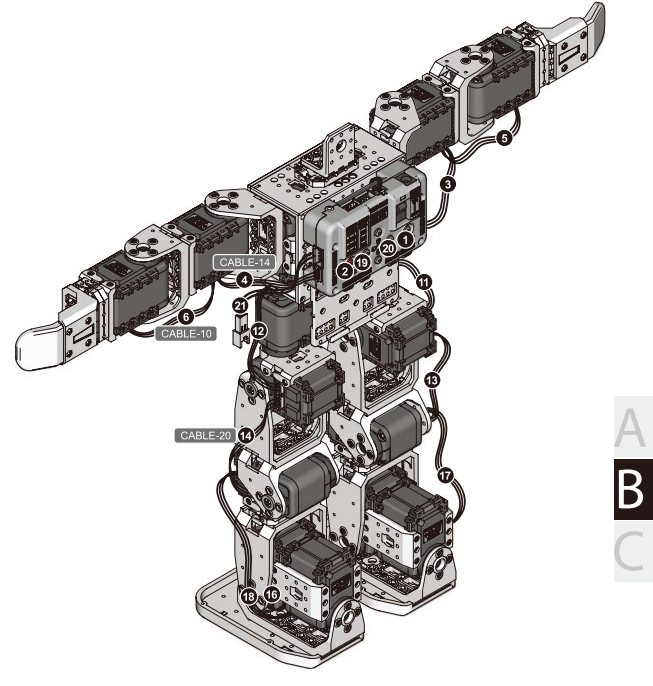
\includegraphics[scale=0.3]{imagenes/RobotTrasero.png}
\caption{Vista trasera del robot con la tarjeta CM-510, tomada del manual del kit Bioloid.}
\label{fig:trasera1}
\end{figure}


En la figura ~\ref{fig:trasera2} se puede observar la estructura del robot con la Arbotix incorporada. En la parte interna del tronco del robot se sitúa el sensor Gyro.

\begin{figure}[hbtp]
\centering
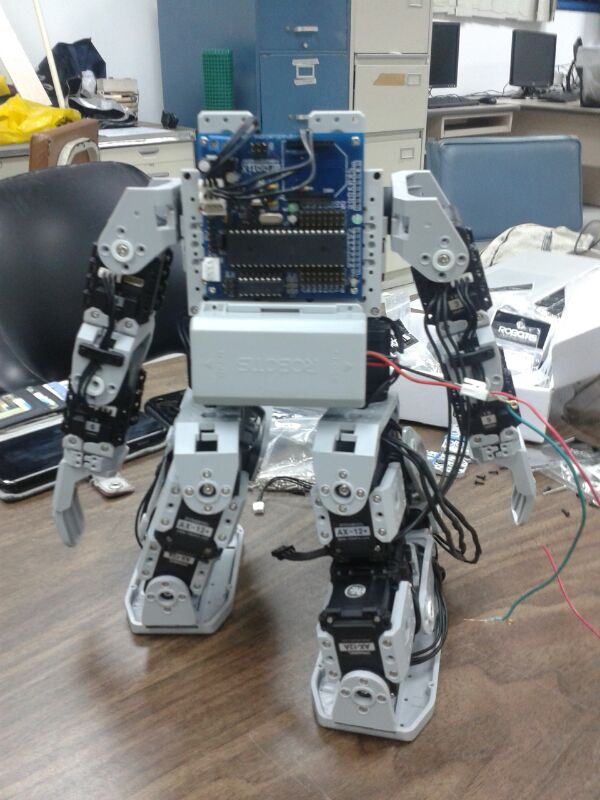
\includegraphics[scale=0.2]{imagenes/traseroDeJunny.jpg}
\caption{Vista trasera del robot con la Arbotix}
\label{fig:trasera2}
\end{figure}


Para el movimiento de la cámara se ha incorporado dos micro servomotores TG9e ya que estos poseen un tama\~no reducido perfecto para acoplarlo en la estructura al igual que su peso, uno para el movimiento horizontal y otro para el vertical. La conexión de uno de estos motores se ilustra en la figura ~\ref{fig:arbotixConectados}, en donde se puede observar que se encuentra conectado al puerto B de los denominados 'Hobby Servo ports'. La cámara ha sido conectada a la Raspberry Pi en el puerto CSI (ver la figura ~\ref{fig:camACSI}). El resultado de estas tres piezas instaladas en el robot se puede apreciar en la figura ~\ref{fig:servosycam}.

%\begin{figure}[hbtp]
%\centering
%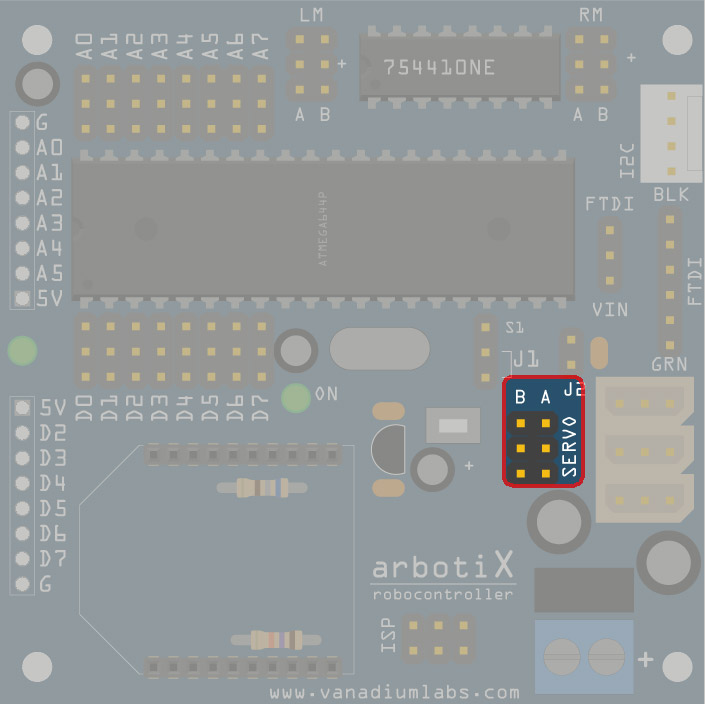
\includegraphics[scale=0.2]{imagenes/arbotix_hobby_servo.jpg}
%\caption{Ilustración de los puertos Hobby de la Arbotix}
%\label{fig:puertosHobby}
%\end{figure}

\begin{figure}[hbtp]
\centering
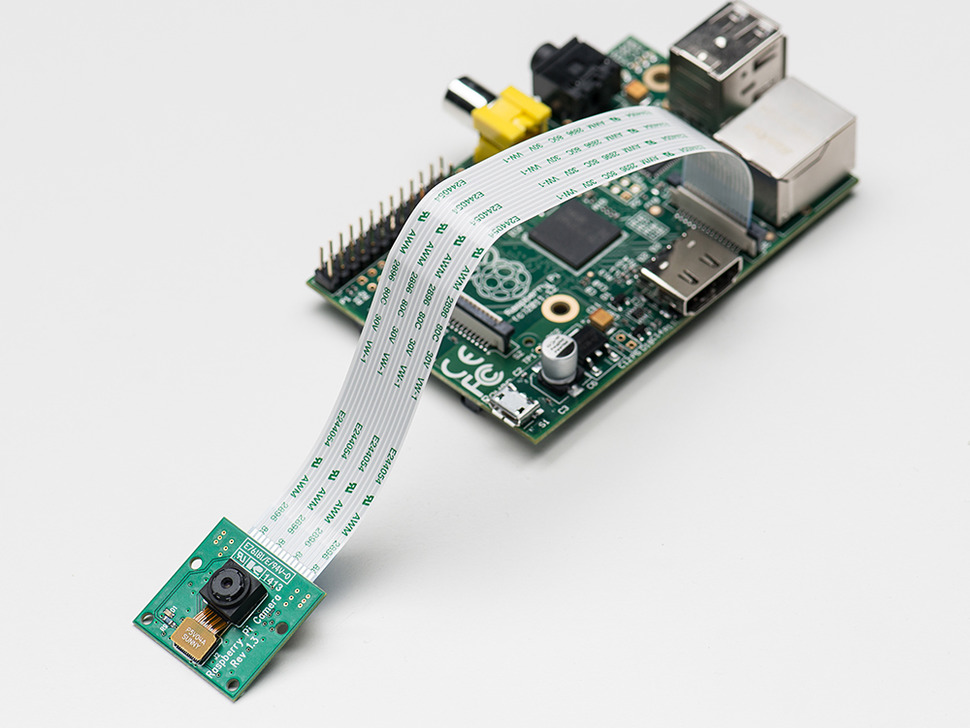
\includegraphics[scale=0.6]{imagenes/raspbCam.jpg}
\caption{C\'amara Raspberry Pi conectada al puerto CSI de la tarjeta}
\label{fig:camACSI}
\end{figure}
 
\begin{figure}[hbtp]
\centering
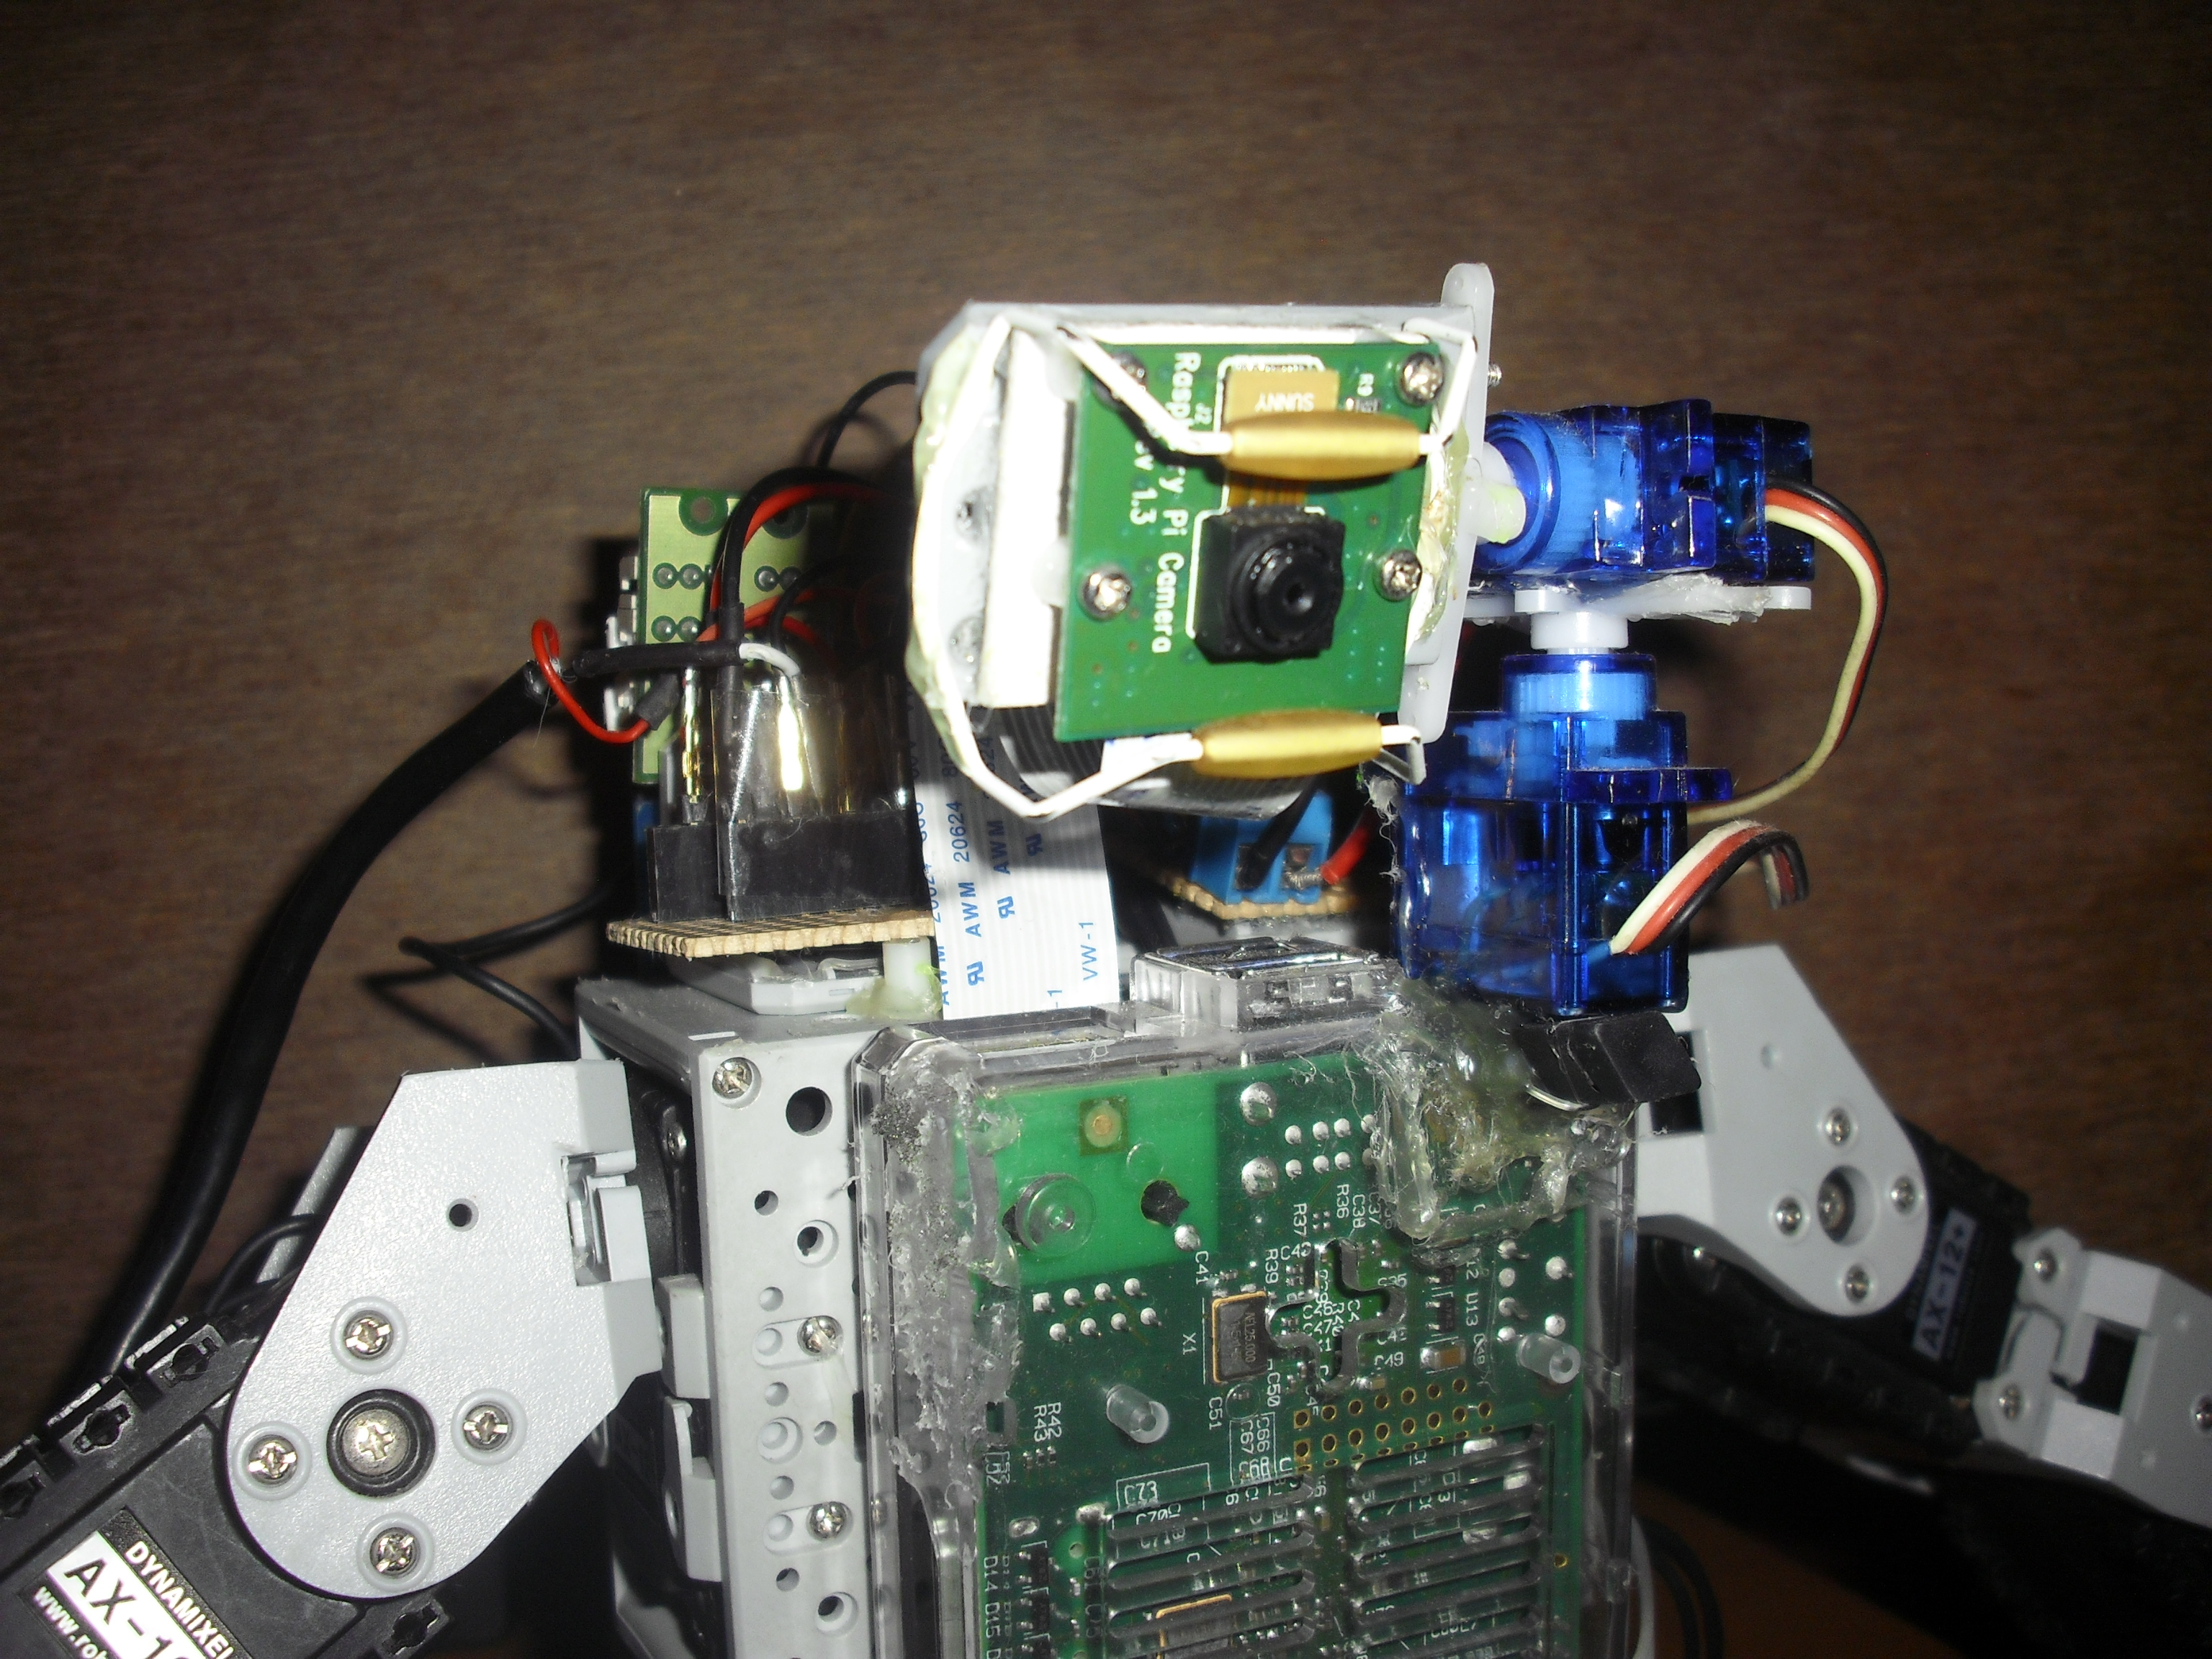
\includegraphics[scale=0.08]{imagenes/servosYcamara.JPG}
\caption{Vista delantera del robot con la cámara y servomotores instalados}
\label{fig:servosycam}
\end{figure}

Los motores Dynamixel se conectan a la controladora Arbotix por medio de los puertos Bioloid de la tarjeta. El diseño de Junny posee cuatro extremidades: dos brazos y dos piernas, por lo que naturalmente, el conjunto de motores, se puede descomponer en cuatro cadenas o series separadas. Sin embargo la Arbotix s\'olo cuenta con tres puertos Bioloid. Se consideró la opción de unir dos extremidades pero ello implicaba limitaciones en el movimiento del robot, por lo tanto se optó por agregar un expansor de puertos Bioloid y así conectar cada extremidad en un puerto diferente. La forma en la que se ha conectado estos motores se ejemplifica en la figura ~\ref{fig:arbotixConectados}. 

\begin{figure}[hbtp]
\centering
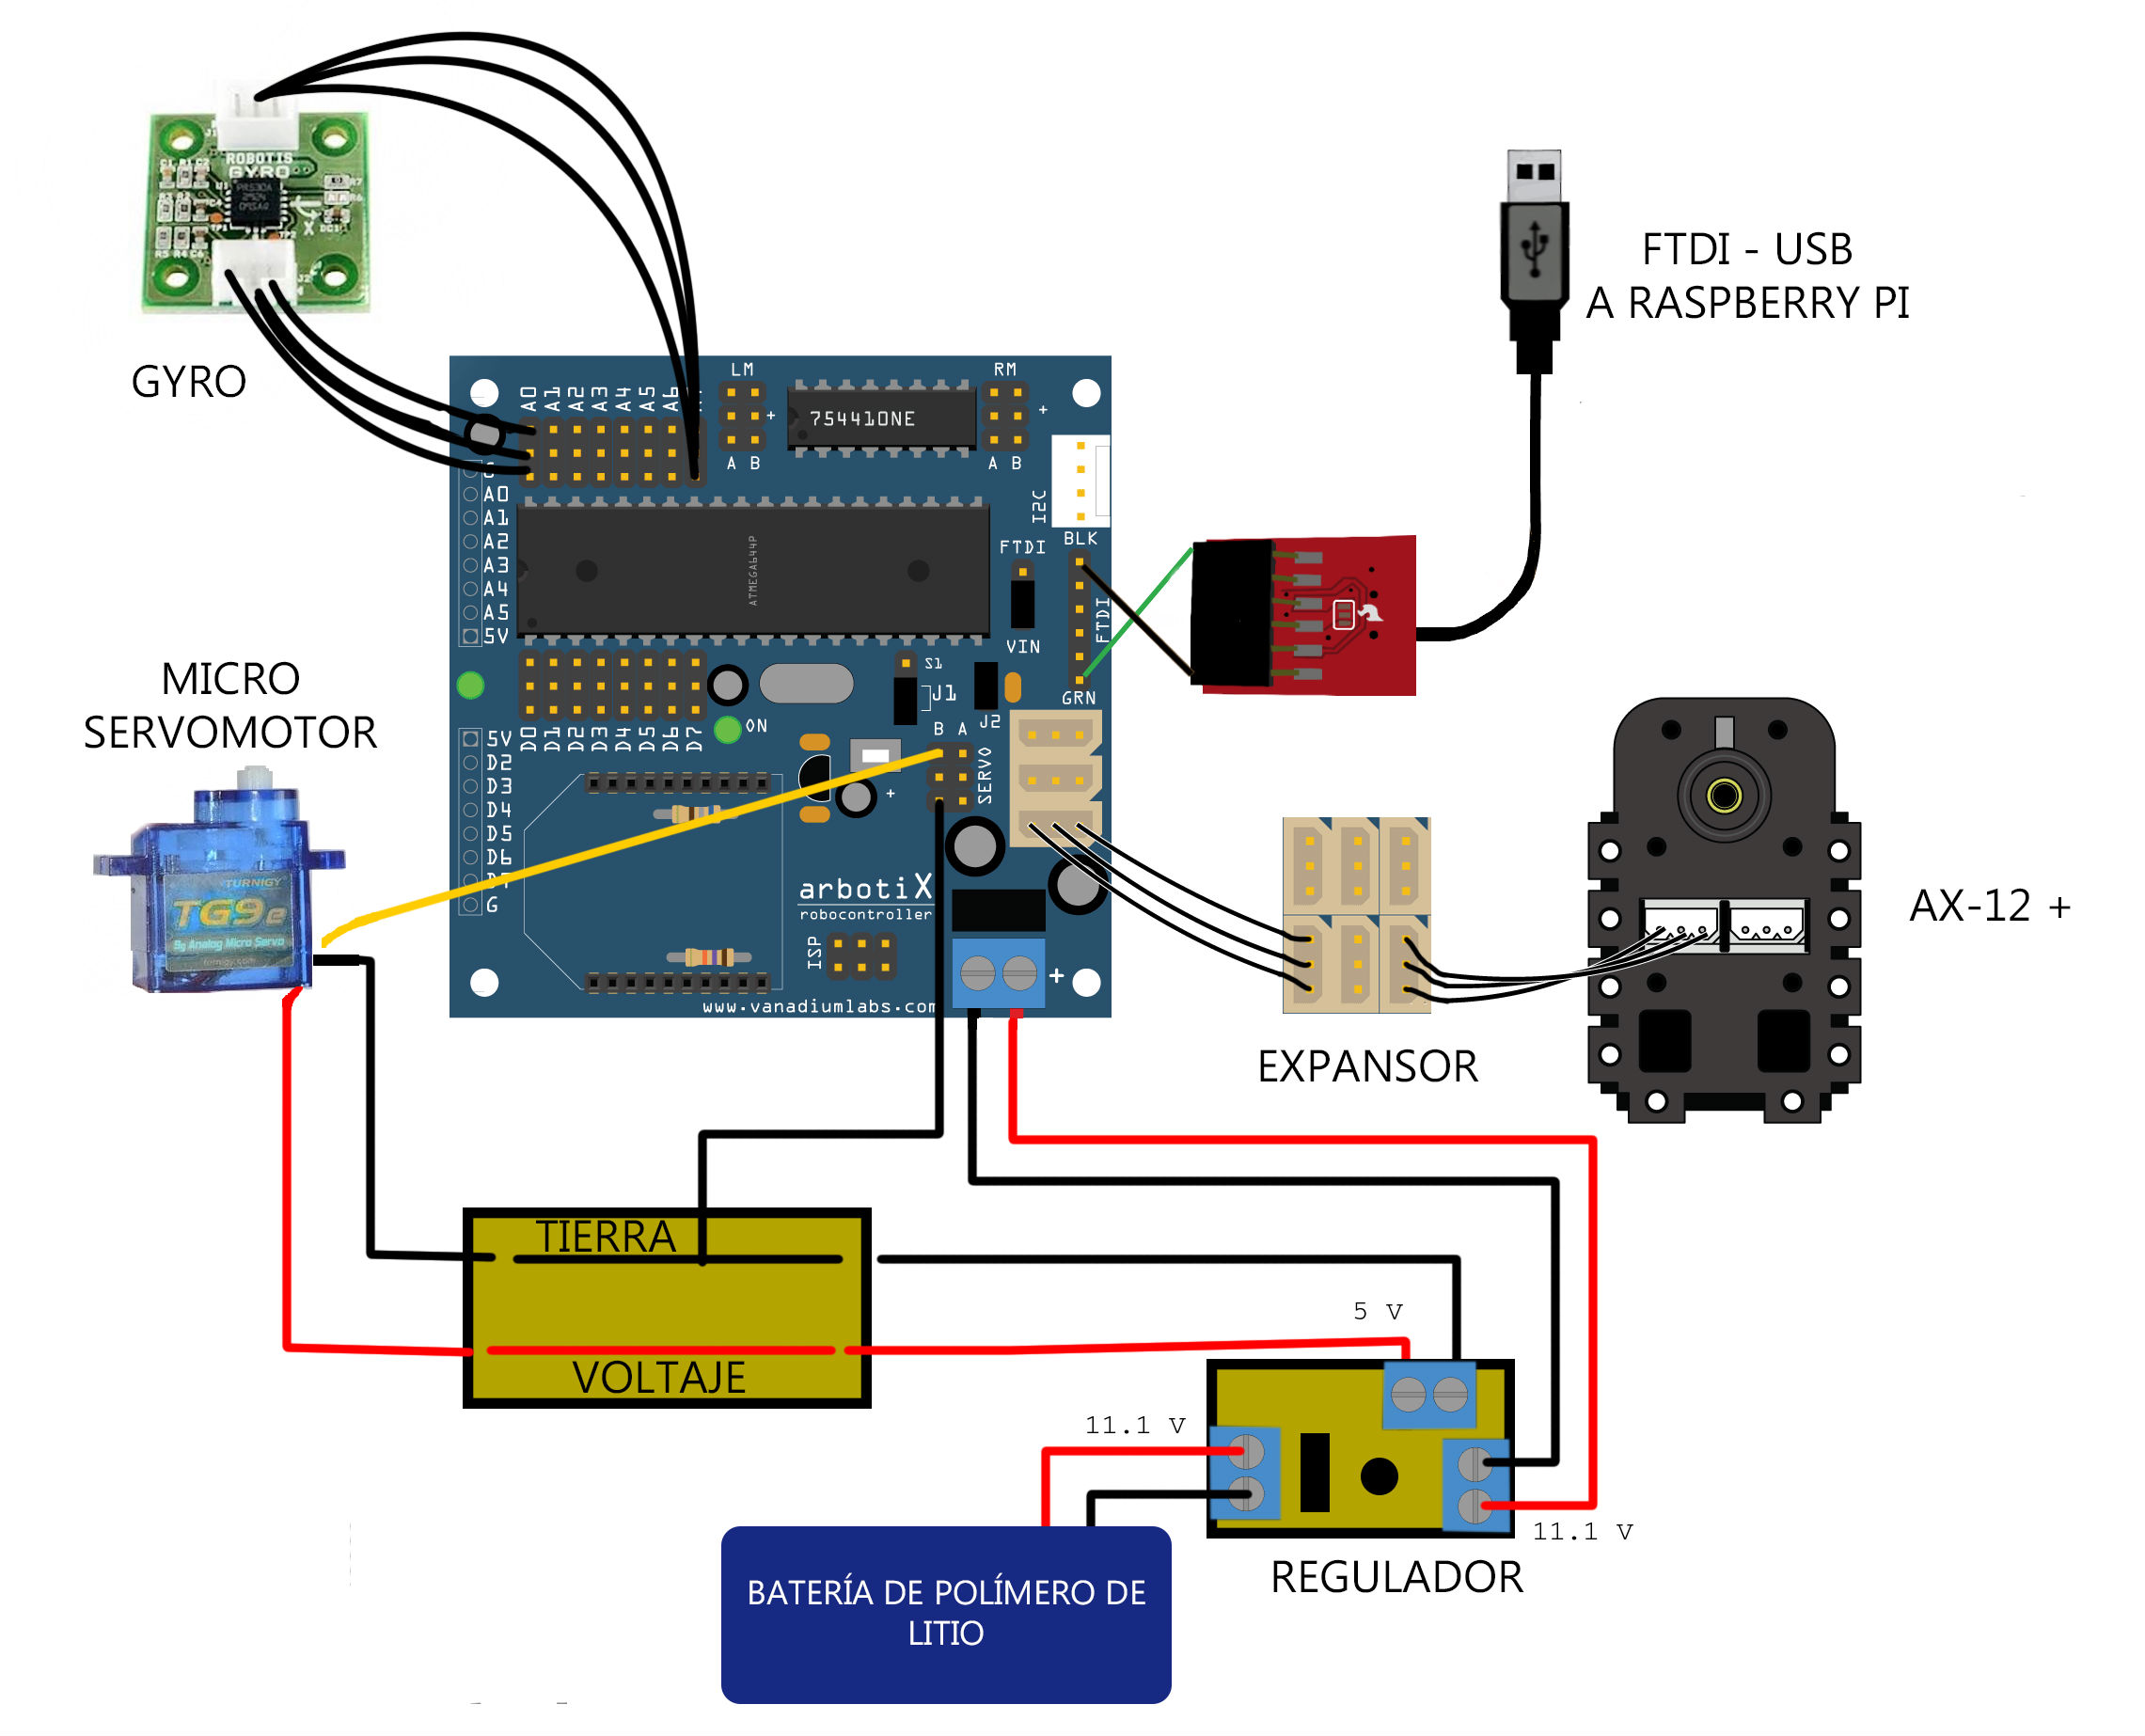
\includegraphics[scale=0.2]{imagenes/arbotix_componentes1.jpg}
\caption{Tarjeta controladora Arbotix y componentes conectados (Imagen referencial: el regulador se encuentra dispuesto en diferente orden)}
\label{fig:arbotixConectados}
\end{figure}

La comunicación de la tarjeta de Arbotix con la computadora, incluso con la Raspberry Pi, se realiza a través del puerto FTDI por medio un chip conectado como lo ilustra la figura ~\ref{fig:arbotixConectados} el USB es conectado a la raspberry Pi y el otro lado al puerto correspondiente en la Arbotix.

Para evitar agregar peso innecesario al robot se decidi\'o solo colocar una sola fuente de poder, se utilizó una batería de polímero de litio de 11.1 V y 1 amp. Por medio del regulador construido alimenta a todos los componentes simultaneamente (ver figura ~\ref{fig:circuito}).



